\documentclass[preprint]{elsarticle}
% vi:spell spelllang=en

\usepackage{hyperref}

\usepackage[english]{babel}
\usepackage[utf8]{inputenc}
\usepackage[T1]{fontenc}

\usepackage{amsmath}  % Maths
\usepackage{amsfonts} % Maths
\usepackage{amssymb}  % Maths
\usepackage{stmaryrd} % Maths (crochets doubles)

\usepackage{url}     % Mise en forme + liens pour URLs
\usepackage{array}   % Tableaux évolués

\usepackage{comment}


\usepackage{prettyref}
\newrefformat{def}{Def.~\ref{#1}}
\newrefformat{fig}{Fig.~\ref{#1}}
\newrefformat{pro}{Property~\ref{#1}}
\newrefformat{pps}{Proposition~\ref{#1}}
\newrefformat{lem}{Lemma~\ref{#1}}
\newrefformat{thm}{Theorem~\ref{#1}}
\newrefformat{sec}{Sect.~\ref{#1}}
\newrefformat{ssec}{Subsect.~\ref{#1}}
\newrefformat{sssec}{Subsect.~\ref{#1}}
\newrefformat{suppl}{Appendix~\ref{#1}}
\newrefformat{eq}{Eq.~\eqref{#1}}
\newrefformat{ex}{Example~\ref{#1}}
\newrefformat{tb}{Table~\ref{#1}}
\newrefformat{rem}{Remark~\ref{#1}}
\def\pref{\prettyref}

\newdefinition{definition}{Definition}
\newdefinition{property}{Property}
\newdefinition{remark}{Remark}
\newdefinition{proposition}{Proposition}
\newdefinition{example}{Example}

\usepackage{tikz}
\newdimen\pgfex
\newdimen\pgfem
\usetikzlibrary{arrows,shapes,shadows,scopes}
\usetikzlibrary{positioning}
\usetikzlibrary{matrix}
\usetikzlibrary{decorations.text}
\usetikzlibrary{decorations.pathmorphing}

% Macros relatives à la traduction de PH avec arcs neutralisants vers PH à k-priorités fixes

% Macros générales
\def\Pint{\textsc{PINT}}

% Notations générales pour PH
\newcommand{\PH}{\mathcal{PH}}
\newcommand{\PHs}{\Sigma}
\newcommand{\PHl}{L}
%\newcommand{\PHp}{\mathcal{P}}
\newcommand{\PHp}{\textcolor{red}{\mathcal{P}}}
\newcommand{\PHproc}{\mathcal{P}}
\newcommand{\PHa}{\PHh}
\newcommand{\PHh}{\mathcal{H}}
\newcommand{\PHn}{\mathcal{N}}

\newcommand{\PHhitter}{\mathsf{hitter}}
\newcommand{\PHtarget}{\mathsf{target}}
\newcommand{\PHbounce}{\mathsf{bounce}}
\newcommand{\PHsort}{\Sigma}

\def\f#1{\mathsf{#1}}
\def\focals{\f{focals}}
\def\play{\cdot}
\def\configs#1{\mathbb C_{#1\rightarrow a}}

%\newcommand{\PHfrappeR}{\textcolor{red}{\rightarrow}}
%\newcommand{\PHmonte}{\textcolor{red}{\Rsh}}

\newcommand{\PHfrappeA}{\rightarrow}
\newcommand{\PHfrappeB}{\Rsh}
%\newcommand{\PHfrappe}[3]{\mbox{$#1\PHfrappeA#2\PHfrappeB#3$}}
%\newcommand{\PHfrappebond}[2]{\mbox{$#1\PHfrappeB#2$}}
\newcommand{\PHfrappe}[3]{#1\PHfrappeA#2\PHfrappeB#3}
\newcommand{\PHfrappebond}[2]{#1\PHfrappeB#2}
\newcommand{\PHobjectif}[2]{\mbox{$#1\PHfrappeB^*\!#2$}}
\newcommand{\PHconcat}{::}
\newcommand{\PHneutralise}{\rtimes}

\def\PHget#1#2{{#1[#2]}}
%\newcommand{\PHchange}[2]{#1\langle #2 \rangle}
\newcommand{\PHchange}[2]{(#1 \Lleftarrow #2)}
\newcommand{\PHarcn}[2]{\mbox{$#1\PHneutralise#2$}}
\newcommand{\PHjoue}{\cdot}

\newcommand{\PHetat}[1]{\mbox{$\langle #1 \rangle$}}


% Notations spécifiques à ce papier
\newcommand{\PHdirectpredec}[1]{\PHs^{-1}(#1)}
\newcommand{\PHpredec}[1]{\f{pred}(#1)}
\newcommand{\PHpredecgene}[1]{\f{reg}({#1})}
\newcommand{\PHpredeccs}[1]{\PHpredec{#1} \setminus \Gamma}

\newcommand{\PHincl}[2]{#1 :: #2}

\def\ctx{\varsigma}
\def\ctxOverride{\Cap}
\def\state#1{\langle #1 \rangle}

% Notations spécifiques aux graphes d'états
%\newcommand{\PHge}{\textcolor{red}{\mathcal{GE}}}
%\newcommand{\PHt}{\mathcal{T}}
%\newcommand{\GE}{\mathcal{GE}}
%\newcommand{\GEt}{\mathcal{T}}
%\newcommand{\GEl}{\PHl}
%\newcommand{\GEa}{\PHa}
%\newcommand{\GEva}[3]{#1 \stackrel{#2}{\longrightarrow} #3}
%\newcommand{\GEval}[3]{#1 \stackrel{#2}{\Longrightarrow} #3}
%\newcommand{\GEget}[2]{\PHget{#1}{#2}}


\def\DEF{\stackrel{\Delta}=}
\def\EQDEF{\stackrel{\Delta}\Leftrightarrow}
\def\SUBSETDEF{\stackrel{\Delta}\subset}

\newcommand{\segmllabel}{\llbracket}
\newcommand{\segmrlabel}{\rrbracket}
\newcommand{\segm}[2]{\segmllabel #1 ; #2 \segmrlabel}
\newcommand{\leqsegm}{\leq_{\segmllabel\segmrlabel}}
\newcommand{\ltsegm}{<_{\llbracket\rrbracket}}

\input{macros-ph}
% Macros spécifiques au Modèle de Thomas / aux RRB

\newcommand{\sN}{\mathbb{N}}

% Notations pour le modèle de Thomas (depuis thèse)
\newcommand{\GRN}{\mathcal{GRN}}
\newcommand{\IG}{\mathcal{G}}
%\def\IG{\mathrm{IG}}
\newcommand{\GRNreg}[1]{\Gamma^{-1}(#1)}
\newcommand{\GRNreslabel}{\mathsf{Res}}
\newcommand{\GRNres}[2]{\GRNreslabel_{#1}(#2)}
%\newcommand{\GRNallres}[1]{\mathsf{Res}_{#1}}
\newcommand{\GRNallres}[1]{\textcolor{red}{\mathsf{Res}_{#1}}}
\newcommand{\GRNget}[2]{\PHget{#1}{#2}}
\newcommand{\GRNstate}[1]{\PHetat{#1}}
\newcommand{\GRNstates}{\mathcal{S}}
\newcommand{\GRNedgef}[4]{#1 \xrightarrow{#2 #3} #4}
\newcommand{\GRNedge}[4]{\GRNedgef{#1}{#2,}{#3}{#4}}
\newcommand{\GRNtrans}[2]{#1 \rightarrow #2}
\newcommand{\uns}{\pm}

\def\levelsl{\mathsf{levels}}
\def\levels#1#2{\levelsl(#1\rightarrow #2)}
\def\ulevels#1#2{\overline{\levelsl}(#1\rightarrow #2)}
%\def\levelsA#1#2{\levels_+(#1\rightarrow #2)}
%\def\levelsI#1#2{\levels_-(#1\rightarrow #2)}
\def\levelsA#1#2{\textcolor{red}{\levelsl_+(#1\rightarrow #2)}}
\def\levelsI#1#2{\textcolor{red}{\levelsl_-(#1\rightarrow #2)}}
%\newcommand{\PHres}{\mathsf{Res}}

\newcommand{\Kinconnu}{\emptyset}
\newcommand{\RRGva}[3]{#1 \stackrel{#2}{\longrightarrow} #3}
\newcommand{\RRGgi}{\mathcal{G}}
\newcommand{\RRGreg}[1]{\RRGgi_{#1}}



%\definecolor{darkred}{rgb}{0.5,0,0}
%\definecolor{lightred}{rgb}{1,0.8,0.8}
%\definecolor{lightgreen}{rgb}{0.7,1,0.7}
\definecolor{darkgreen}{rgb}{0,0.5,0}
%\definecolor{darkyellow}{rgb}{0.5,0.5,0}
%\definecolor{lightyellow}{rgb}{1,1,0.6}
%\definecolor{darkcyan}{rgb}{0,0.6,0.6}
%\definecolor{darkorange}{rgb}{0.8,0.2,0}

%\definecolor{notsodarkgreen}{rgb}{0,0.7,0}

%\definecolor{coloract}{rgb}{0,1,0}
%\definecolor{colorinh}{rgb}{1,0,0}
\colorlet{coloract}{darkgreen}
\colorlet{colorinh}{red}
%\colorlet{coloractgray}{lightgreen}
%\colorlet{colorinhgray}{lightred}
%\colorlet{colorinf}{darkgray}
%\colorlet{coloractgray}{lightgreen}
%\colorlet{colorinhgray}{lightred}

%\colorlet{colorgray}{lightgray}


\tikzstyle{grn}=[every node/.style={circle,draw=black,outer sep=2pt,minimum
                size=15pt,text=black}, node distance=1.5cm]
\tikzstyle{act}=[->,draw=black,thick,color=black]
\tikzstyle{inh}=[>=|,-|,draw=black,thick, text=black,label]
%\tikzstyle{inh}=[>=|,-|,draw=colorinh,thick, text=black,label]
%\tikzstyle{act}=[->,>=triangle 60,draw=coloract,thick,color=coloract]
%\tikzstyle{inhgray}=[>=|,-|,draw=colorinhgray,thick, text=black,label]
%\tikzstyle{actgray}=[->,>=triangle 60,draw=coloractgray,thick,color=coloractgray]
\tikzstyle{inf}=[->,draw=colorinf,thick,color=colorinf]
%\tikzstyle{elabel}=[fill=none, above=-1pt, sloped,text=black, minimum size=10pt, outer sep=0, font=\scriptsize,draw=none]
\tikzstyle{elabel}=[fill=none,text=black, above=-2pt,%sloped,
minimum size=10pt, outer sep=0, font=\scriptsize, draw=none]
%\tikzstyle{elabel}=[]
\tikzstyle{sg}=[every node/.style={outer sep=2pt,minimum
                size=15pt,text=black}, node distance=2cm]



% Commandes À FAIRE
\usepackage{color} % Couleurs du texte
\newcommand{\todo}[1]{\textcolor{red}{\textbf{[TODO: #1]}}}
%\newcommand{\rewrite}[1]{\rewriteil{REWRITE: #1}}


\def\modMF#1{\textcolor{teal}{#1}}
\def\modLP#1{\textcolor{magenta}{#1}}
\def\modMM#1{\textcolor{blue}{#1}}
\def\modOR#1{\textcolor{olive}{#1}}



% Id est
\newcommand{\ie}{i.e.~}

% Césures
\hyphenation{pa-ra-me-tri-za-tion}
\hyphenation{pa-ra-me-tri-za-tions}



\begin{document}

\begin{frontmatter}

\title{\modLP{Identification of} Biological Regulatory Networks from Process Hitting models}
%\\\rewriteil{Or possibly: “Complementarity between PH, IG and Thomas modeling”}

\author[irccyn,nii]{Maxime Folschette}
\ead{Maxime.Folschette@irccyn.ec-nantes.fr}
\author[lri]{Lo\"ic Paulev\'e}
\author[nii]{Katsumi Inoue}
\author[irccyn,nii]{Morgan Magnin}
\author[irccyn]{Olivier Roux}

\address[irccyn]{LUNAM Universit\'e, \'Ecole Centrale de Nantes, IRCCyN UMR CNRS 6597\\
(Institut de Recherche en Communications et Cybern\'etique de Nantes)\\
1 rue de la No\"e - B.P. 92101 - 44321 Nantes Cedex 3, France.}
\address[nii]{National Institute of Informatics,\\
2-1-2, Hitotsubashi, Chiyoda-ku, Tokyo 101-8430, Japan.}
\address[lri]{CNRS, Laboratoire de Recherche en Informatique UMR CNRS 8623\\
Universit\'e Paris-Sud, 91405 Orsay Cedex, France}


\begin{abstract}
\modOR{Qualitative formalisms offer a well-established alternative to the more traditionally used differential equation models of Biological Regulatory Networks (BRNs). These formalisms, introduced by Kauffman, Glas and Thomas, led to numerous theoretical works and practical tools to understand emerging behaviors.} \modMM{The analysis of dynamics of very large models is however a rather hard problem, which led us to previously introduce a new framework:} the Process Hitting (PH), \modMM{which} \modLP{is a particular class of Indeterministic Asynchronous Automata
Network (or safe Petri nets).} \modMM{Its major advantage lies in the efficiency of several static analyses recently designed to assess dynamical properties, making it possible to tackle very large models.}

\modLP{In this paper, we address the formal identification of qualitative
models of Biological Regulatory Networks (BRNs) from PH models.}
First, the inference of the Interaction Graph (IG) from a PH model
\modLP{summarizes the signed influences between the components} that are effective for the dynamics.
Second, we provide the inference of all Ren\'e Thomas models of BRNs 
that are compatible with a given PH.
As the PH allows the specification of indeterministic interactions between
components, our inference emphasizes the ability of PH to deal with large BRNs with incomplete knowledge
on interactions, where Thomas' approach fails because of the combinatorics of parameters.

The inference of corresponding Thomas models is \modLP{implemented} using Answer Set Programming,
which allows an efficient enumeration of (possibly numerous) compatible parametrizations.
\end{abstract}

\begin{keyword}
qualitative modeling \sep
model abstraction \sep
interaction graph \sep
René Thomas' parameters \sep
answer set programming
\end{keyword}

\end{frontmatter}


% vim:spell spelllang=en:
\section{Introduction}\label{sec:intro}

As regulatory phenomena play a crucial role in biological systems, they need to be studied accurately.
Biological Regulatory Networks (BRNs) consist in sets of either positive or negative mutual effects between the components.
With the purpose of analyzing these systems, they are often modeled as graphs which make it possible to determine the possible evolutions of all the interacting components of the system.
\modOR{Besides continuous models of physicists, generally designed through systems of ordinary differential equations, modeling regulatory networks by means of Boolean networks has become popular in the wake of Kauffman work \cite{kauffman1969metabolic}.
We based our work on a logical formalism developed by Ren\'e Thomas from 1973 \cite{Thomas73} that generalizes upon Boolean networks in the sense that it allows variables to have more than two values and transitions between states to occur asynchronously.}

In this approach, the different levels of a component, such as concentration or expression levels, are abstractly represented by (positive) integer values and transitions between these levels may be considered as instantaneous.
Hence, qualitative state graphs may be derived from which we are able to formally find out all the possible behaviors expressed as sequences of transitions between these states.
Nevertheless, these dynamics can be precisely established only with regard to some discrete parameters,
hereafter called ``Thomas' parameters'',
which stand for kinds of ``focal points'', \ie the evolutionary tendency from each state and depending on the set of the other currently interacting components.
%resources in this very state, that is, the set of the other currently interacting components.
%Hereafter, we refer to these discrete parameters as Thomas' parameters.

Thomas' modeling has motivated numerous works around the link between the Interaction Graph (IG)
(summarizing the global influences between components) and the possible dynamics (e.g.,
\cite{RiCo07,RRT08}),
model reduction (e.g., \cite{Naldi09}), formal checking of dynamics (e.g., \cite{Richard06,Naldi07}), 
and the incorporation of time (e.g., \cite{Siebert06,Ahmad08}) and probability
(e.g., \cite{Twardziok10-CMSB}) dimensions, to name but a few.

While the formal checking of dynamical properties is often limited to small networks because of the
state graph explosion, an other major drawback of this framework is the difficulty to
specify Thomas' parameters, especially for large networks. \modOR{Other works have also been carried out with the aim of dealing with large systems (e.g. \cite{Corblin200991,Bollman2007,Delaplace2012, 10.1371/journal.pone.0007992}).} \modMM{Because of the complexity of such systems, these works generaly focus on some restricted properties,} \modOR{as finding out steady states.} 
%\todo{The reviewer proposes to nuance this with several papers:
%\begin{itemize}
%  \item Corblin, F., Tripodi, S., Fanchon, E., Ropers, D., \& Trilling, L. (2009).
%    A declarative constraint-based method for analyzing discrete genetic
%    regulatory networks. Bio Systems, 98(2), 91104.
%  \item Bollman, D., Coln-Reyes, O., \& Orozco, E. (2007). Fixed points in
%    discrete models for regulatory genetic networks. EURASIP journal on
%    bioinformatics \& systems biology, 2007, 97356.
%  \item Delaplace, F., Klaudel, H., Melliti, T., \& Sen, S. (2012). Analysis
%    of modular organisation of interaction networks based on asymptotic
%    dynamics. In D. Gilbert \& M. Heiner (Eds.), CMSB 2012
%  \item Scalable Steady State Analysis of Boolean Biological Regulatory Net-
%    works Ay F, Xu F, Kahveci T (2009) Scalable Steady State Analysis
%    of Boolean Biological Regulatory Networks. PLoS ONE 4(12): e7992.
%\end{itemize}
%This can be in turn be nuanced as some papers only focus on rather specific aspects (like steady-states for instance).}

In order to address the formal analysis of additional dynamical properties \modMM{(e.g., state reachabilities)} within very large BRNs, we recently
introduced in \cite{PMR10-TCSB} a new formalism, named the \emph{Process Hitting} (PH), to model
concurrent systems having components with a few qualitative levels.
A PH model describes, in an atomic manner, the possible evolutions of a process (representing one
component at one level) triggered by the hit of at most one other process in the system.
This framework can be seen as a special class of formalisms like Petri Nets or Communicating Finite
State Machines, where the arity and the effect of synchronizations between components are
restricted.
Thanks to the particular structure of interactions within a PH, very efficient static analysis
methods have been developed to over- and under-approximate reachability properties making tractable
the formal analysis of the qualitative dynamics of BRNs with hundreds or thousands of components,
which was impossible with other state-of-the-art approaches \cite{PMR12-MSCS,PAK13-CAV,FPMR13-CS2Bio}.
 
The PH is suitable to model BRNs with different levels of abstraction in the specification of
cooperations (associated influences) between components. \modOR{The concept of cooperation refers to the} \modMM{way two (or more) components jointly influence a third one. In other words, it captures the logical functions stating how} \modOR{various elements coalesce and act together upon an other element among the network.}
\modLP{In particular, PH allows to specify partial (non-deterministic) cooperations that superpose the dynamics of 
candidate fully-specified (deterministic) cooperations.
This permit to model BRNs with a partial knowledge on precise evolution functions for components
by capturing the largest (the most general) dynamics, without a combinatorics enumeration of
compatible Thomas models.}

\medskip

The aim of this paper is to formally establish links between several layers suited for specifying the
qualitative dynamics of BRNs, namely:
the Interaction Graph (IG), referencing the sign of direct regulations between components;
the Process Hitting (PH), which permits to specify the qualitative dynamics of the system with
various degrees of knowledge for joint regulations;
and Thomas' parameters, which completely specify the functions governing the evolution of
components.
Another motivation for the work depicted in this paper is that it constitutes an important step
to go further in the study of large biological regulatory networks systems beyond simple analysis:
it makes it possible to partly control some behaviors.
Indeed, when one wants to modify some behaviors
(e.g.~so as to avoid the reachability of some states or to create stable states)
we intend to be able to get upstream the results in accordance at the regulatory level.
The outcome of the present work is that we could make such changes on the PH model
and then recover afterwards the BRN corresponding to the transformed behavioral system.
In a more general framework and in an interesting way,
we should be able to synthesize families of BRN having some featuring behavioral properties.

Firstly, we derive rules that, given a PH model, infer the IG corresponding to the dynamics of the
encoded BRN.
The obtained IG relates only components that have actual influence in the dynamics.
This typically results into IGs that contain less interactions than an hypothetical starting prior
IG, as the specification of component evolutions may reveal non-functional regulations.
Based on the derived IG, various static analysis allows to conclude on global properties
of the system dynamics (see \cite{PR11-SASB} for a short survey).
The most known are the Thomas' conjectures (that have been proved since,
e.g.~\cite{RRT08,RiCo07,Richard2010378}
for Boolean and discrete networks),
which relate the absence of
positive cycle to the impossibility for multi-stationarity (distinct attractors),
and the absence of negative cycle to the impossibility for oscillatory behaviors.

Second, we tackle the inference of Thomas' parameters that are compatible with a given PH
model, \ie that fully specify the evolution of components while respecting the cooperations
specified in PH.
More formally, the resulting BRN dynamics is ensured to be included in the PH dynamics: any
transition in the (asynchronous) Thomas model exists in the PH model.
In practice, the number of compatible Thomas parameters can be huge for large networks where only a
few cooperations are specified.
This highlights that the PH is suitable to analyze dynamics of large-scale networks
where the knowledge on cooperations is often incomplete:
instead of dealing with a possibly non-tractable number of Thomas models, one can already capture
precise dynamical features using a single PH model which gathers all the plausible dynamics.

Finally, we discuss on an implementation of these inference schemes using Answer Set
Programming (ASP) \cite{Baral03},  which turns out to be effective for these enumerative searches.
The whole method is also applied to the biological model of ERBB receptor-regulated G1/S transition,
containing 20 components,
which allows to detail how joint actions can be defined inside a PH model in order
to refine its dynamics, and study a more precise class of underlying Thomas models.
%\todo{describe application}

Our work is related to the approach of \cite{Khalis09} which relies on temporal logic, and \cite{20646302,DBLP:conf/ipcat/CorblinFTCT12} which also uses constraint programming.
Both aim at determining a class of models which are consistent with available partial data on the regulatory structure and dynamical properties.
%These classes are built in order to infer properties common to some studied models.
%In our approach, we intend to focus on the Thomas' parameters inference
Our method is based on a model rather than on constraints, which allows to define some properties on the system structure (such as cooperations).
Furthermore, we claim that we are able to deal with larger biological networks.
Finally, it must be noticed that we are not interested in this paper in the derivation of one PH
from a BRN (which was previously described in \cite{PMR10-TCSB}) but, on the contrary, in finding
out a set of BRNs from one PH.

The contributions presented in this paper significantly extend and improve the preliminary results
introduced in \cite{FPIMR12-CMSB}.
In addition to the improvement of the efficiency and accuracy of the IG inference, we have added support for
\modLP{non-monotonous} regulations, that are regulations being positive or negative depending on a particular
context.
This allows to apply our methodology to a wider class of models.
Furthermore, some parts have been completely rewritten in order to explain more precisely the efficiency of the ASP implementation,
and give a new detailed biological application of our work.

\paragraph{Outline}
\pref{sec:frameworks} recalls the PH and Thomas frameworks;
\pref{sec:infer-IG} defines the IG inference from PH;
\pref{sec:infer-K} details the parameters inference and the enumeration of Thomas parametrizations compatible with a PH;
\pref{sec:impl} discusses the implementation of the latter in ASP.
\pref{sec:examples} illustrates our method on a biological model
and discusses its applicability on large models.

\paragraph{Notations}
$\segm{i}{j}$ is the set of integers $\{ i, i+1, \dots, j \}$.


\section{Frameworks}\label{sec:frameworks}
\input{parts-ph}
% vim:spell spelllang=en
\subsection{Thomas' modeling}

\todo{Name Kaufman as the creator of BRNs.}

We concisely present Thomas' modeling of a Biological Regulatory Network (BRN) and its dynamics, merely inspired by
\cite{Richard06,BernotSemBRN}.
In order to enlarge the class of Thomas' models compatible with PH dynamics (w.r.t.~the presented
inference),
we propose the notion of unsigned edge modeling an interaction whose nature (activation or inhibition) is undetermined,
and we extend the classical parametrization formalism by setting parameters to intervals of values instead of single values.
We briefly discuss these additions.

\medskip

Thomas' formalism lies on two complementary descriptions of the system. First, the
\emph{Interaction Graph} (IG) models the structure of the system by defining the components'
mutual influences and the conditions of these influences.
The \emph{parametrization} then specifies the levels towards which tends a component when a given
configuration of its regulators applies.

The IG is composed of nodes ($a$, $b$, $c$, …) that represent components,
and edges ($\GRNedge{a}{s}{t}{b}$, …) labeled with a sign ($s$) and a threshold ($t$) that stand for regulations between these components (\pref{def:ig}).
The activity, concentration rate or presence of each component in a given state of the system is modeled by an abstract discrete value called \emph{expression level}.
The maximum expression level of a component $a$ is denoted $l_a$.
The sign of an edge denotes the kind of regulation it models: it can be positive ($+$), negative ($-$) or unsigned ($\uns$),
the latter meaning that the nature of the regulation cannot be reduced to a simple activation or inhibition.
Regarding the dynamics, an edge $\GRNedge{a}{s}{t}{b}$ states that $a$ influences the evolution of $b$ in a certain way when its expression level is above or equal to the threshold $t$;
when its expression level is strictly below this threshold, another kind of influence is expressed, which usually consists of the opposite influence.
%For a regulation to take place (activation or inhibition), the expression level of its head component has to be higher than its threshold;
%otherwise, the opposite influence is expressed.
The uniqueness of each regulation is forced, in order to make the following sections simpler.
The purpose of unsigned edges is discussed at the end of the current section.

\todo{Discuss about the meaning of signs (especially $+$ and $-$) and their link with parameters.
Especially, these signs introduce redundancy (and possibly contradiction) with the parameters.
\begin{itemize}
  \item We can discuss more about the choice we made here: the signs are only informative
    (it eases the read of the IG), but are used as a basis for the parameters enumeration;
  \item The reviewer suggests to remove signs, or only present them as an abstraction of the monotonicity assumption, given the levels and parameters of a BRN;
  \item It is also possible to add the monotonicity assumption in the definition of a BRN to avoid contradictions.
\end{itemize}}

\begin{definition}[Interaction Graph]
\label{def:ig}
An \emph{Interaction Graph} (IG) is a couple $\IG = (\Gamma, E)$ with $\Gamma$ the finite set of \emph{components},
and $E$ the finite set of \emph{regulations} between two nodes, labeled with a \emph{sign} and a \emph{threshold}:
$$E \DEF \{ \GRNedge{a}{s}{t}{b}, \ldots \mid a, b \in \Gamma \wedge s \in \{ +, -, \uns \} \wedge t \in \segm{1}{l_a}\} \enspace,$$
where a regulation from $a$ to $b$ is uniquely referenced:
$$\forall \GRNedge{a}{s}{t}{b} \in E, \forall \GRNedge{a}{s'}{t'}{b} \in E, s = s' \wedge t = t' \enspace.$$
\end{definition}

\todo{The notation $\GRNreg{b}$ is poorly chosen; should be replaced by $E^{-1}(b)$ for instance.}

Given this definition, we denote as a shortcut:
$E_s \DEF \{ \GRNedge{a}{s}{t}{b} \in E \}$ for $s \in \{ +, -, \uns \}$.
Furthermore, for all component $b \in \Gamma$, we denote $\GRNreg{b}$ the set of its regulators as defined in \pref{eq:grn-regulators}.
\begin{align}
\label{eq:grn-regulators}
  \GRNreg{b} \DEF \{ a\in\Gamma\mid \exists \GRNedge{a}{s}{t}{b} \in E \}
\end{align}
Then, for all component $a$ regulating $b$,
\ie if $\GRNedge{a}{s}{t}{b} \in E$,
we denote $\levels{a}{b}$ (resp.~$\ulevels{a}{b}$) the interval of expression levels of $a$ above (resp.~below) the threshold $t$ (\pref{def:levels}).
For all expression levels of $a$ that belong to $\levels{a}{b}$, $a$ is expected to have the influence corresponding to the sign $s$ on $b$;
for all expression levels belonging to $\ulevels{a}{b}$, the opposite influence is expected.
This definition holds because of the uniqueness of the edge $\GRNedge{a}{s}{t}{b}$.

\begin{definition}[Effective levels ($\levelsl$)]\label{def:levels}
If $\GRNedge{a}{s}{t}{b} \in E$, we define:
%Let $b \in \Gamma$ and $a \in \GRNreg{a}$; we define:
$$\levels{a}{b} \DEF \segm{t}{l_a} \quad \text{and} \quad \ulevels{a}{b} \DEF \segm{0}{t-1} \enspace.$$
\end{definition}

\begin{example}
\pref{fig:runningBRN}(left) represents an Interaction Graph $(\Gamma,E)$ where
$\Gamma = \{a, b, c\}$, with $l_a = 2$ and $l_b = l_c = 1$,
and:
\begin{align*}
  E_+ &= \{\GRNedgef{b}{+}{1}{a}, \GRNedgef{c}{+}{1}{a}\} &
  E_\uns &= \emptyset \\
  E_- &= \{\GRNedgef{a}{-}{2}{b}\}
\end{align*}
Hence:
\begin{align*}
  \GRNreg{a} &= \{ b, c \} &
  \GRNreg{b} &= \{ a \} \\
  \GRNreg{c} &= \emptyset
\end{align*}
We also have especially:
\begin{align*}
  \levels{a}{b} &= \segm{2}{2} & \ulevels{a}{b} &= \segm{0}{1}
\end{align*}
\end{example}

\begin{figure}[t]
\begin{minipage}{0.4\linewidth}
\centering
\scalebox{1.2}{
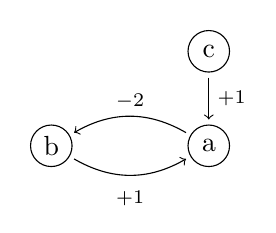
\begin{tikzpicture}[grn]
  \path[use as bounding box] (-0.3,-0.75) rectangle (2.5,1.5);
  \node[inner sep=0] (a) at (2,0) {a};
  \node[inner sep=0] (b) at (0,0) {b};
  \node[inner sep=0] (c) at (2,1.2) {c};
  \path[->]
    (b) edge[bend right] node[elabel, below=-2pt] {$+1$} (a)
    (c) edge node[elabel, right=-2pt] {$+1$} (a)
    (a) edge[bend right] node[elabel, above=-5pt] {$-2$} (b);
\end{tikzpicture}
}
\end{minipage}
\begin{minipage}{0.6\linewidth}
\centering
\begin{align*}
  K_{a,\emptyset} &= \segm{0}{0} & K_{b,\emptyset} &= \segm{0}{1} \\
  K_{a,\{b\}} &= \segm{1}{1} & K_{b,\{a\}} &= \segm{0}{0} \\
  K_{a,\{c\}} &= \segm{1}{1} &&\\
  K_{a,\{b,c\}} &= \segm{2}{2} & K_{c,\emptyset} &= \segm{0}{1}
\end{align*}
\end{minipage}
\caption{\label{fig:runningBRN}
  (left)
  IG example.
  Components are represented by nodes labeled with a name
  and regulations by edges labeled with their sign and threshold.
  For instance, the edge from $b$ to $a$ is labeled $+1$, which stands for: $\GRNedgef{b}{+}{1}{a}$.
  This means that if the expression level of $b$ is equal to (\ie above) 1, then $b$ activates $a$;
  otherwise, $b$ inhibits $a$.
  (right)
  Example parametrization on the left IG.
}
\end{figure}

A \emph{state} $s$ of an IG $(\Gamma, E)$ is an element in $\GRNstates \DEF \prod_{a \in \Gamma} \segm{0}{l_a}$.
$\GRNget{s}{a}$ refers to the level of component $a$ in $s$.
For each possible state, the set of \emph{resources} of a given component
is the set of regulators of this component whose expression level is above the threshold of the regulation (\pref{def:resources}).
In other words, in every state $s$, a regulator $b$ of a component $a$
is either a resource (if $\GRNget{s}{b} \in \levels{b}{a}$)
or not a resource (if $\GRNget{s}{b} \in \ulevels{b}{a}$).
%For each possible state, all regulators of a component $a$ can be divided into
%\emph{activators} and \emph{inhibitors}, given their type of interaction and expression level,
%referred to as the \emph{resources} of $a$ in this state (\pref{def:resources}).
Relying on this observation, the specificity of Thomas' approach lies in the use of discrete \emph{parameters} to represent the
focal level interval towards which the component will evolve in every configuration of the resources (\pref{def:param}).

\begin{definition}[Resources ($\GRNreslabel$)]\label{def:resources}
For a given component $a \in \Gamma$ and a state $s \in \GRNstates$,
the set of regulators of $a$ whose level in $s$ is above the related threshold %to regulate $a$
is called the set of \emph{resources} of $a$ in $s$ and is noted $\GRNres{a}{s}$:
$$\GRNres{a}{s} \DEF \{ b \in \GRNreg{a} \mid \GRNget{s}{b} \in \levels{b}{a} \}$$
\end{definition}

\begin{definition}[Parameter $K_{a,\omega}$ and Parametrization $K$]\label{def:param}
For a given component $a \in \Gamma$, and $\omega \subset \GRNreg{a}$ a set of regulators of $a$,
the \emph{parameter} $K_{a,\omega} = \segm{i}{j}$ is a non-empty interval with with $0 \leq i \leq j \leq l_a$.
The complete map $K$ of parameters on $\IG$ is called a \emph{parametrization} on $\IG$.
\end{definition}

%\todo{Discuss on the widespread use of discrete parameters + binary resources}
An IG and a parametrization make up a complete BRN.
The purpose of intervals as parameters is discussed at the end of this section.
Regarding the dynamics, an interval parameter $K_{a,\omega}$ is the set of values towards which $a$ will tend
in the states where its resources are exactly the regulators in $\omega$.
%as defined in the asynchronous dynamics of \pref{def:dynamics}.
%At last, \pref{def:dynamics} gives the asynchronous dynamics of a BRN using Thomas' parameters.
Indeed, from a given state $s$, a transition to another state $s'$ is possible provided that
exactly one component $a$ evolves of one expression level towards the closest value of the interval $K_{a,\GRNres{a}{s}}$,
as stated by the definition of the transition relation $\GRNtrans{s}{s'}$ (\pref{def:dynamics}).
However, $a$ cannot evolve if its expression level already belongs to the interval $K_{a,\GRNres{a}{s}}$.

\begin{definition}[Asynchronous dynamics ($\GRNtrans{}{}$)]\label{def:dynamics}
The dynamics of a BRN using Thomas' parameters is given by the transition relation $\GRNtrans{}{}\ \in \GRNstates \times \GRNstates$ defined by:
\begin{align*}
  \forall s, s' \in \GRNstates, \GRNtrans{s}{s'} &\Longleftrightarrow \exists a \in \Gamma,
  \GRNget{s}{a} \notin K_{a, \GRNres{a}{s}} \wedge \GRNget{s'}{a} = \GRNget{s}{a} + \delta^a(s) \\
    & \qquad\quad \wedge \forall b \in \Gamma, b \neq a \Rightarrow \GRNget{s}{b} = \GRNget{s'}{b}
\end{align*}
with: $\delta^a(s) = 
  \begin{cases}
    +1 & \text{if } \GRNget{s}{a} < K_{a, \GRNres{a}{s}} \\
    -1 & \text{if } \GRNget{s}{a} > K_{a, \GRNres{a}{s}} \\
  \end{cases}$
\end{definition}
The notations “$<$” and “$>$” comparing an integer and an interval were defined at the end of \pref{sec:intro}.



\begin{example}
\pref{fig:runningBRN}(right) gives a Parametrization on the IG of \pref{fig:runningBRN}(left).
In this BRN, the following transitions are possible given the semantics defined in \pref{def:dynamics}:
$$\GRNstate{a_0, b_1, c_1} \rightarrow \GRNstate{a_1, b_1, c_1} \rightarrow \GRNstate{a_2, b_1, c_1} \rightarrow
\GRNstate{a_2, b_0, c_1} \rightarrow \GRNstate{a_1, b_0, c_1} \enspace,$$
where $a_i$ denotes the component $a$ at level $i$.
This sequence of states ends in a steady state: no evolution is possible in $\GRNstate{a_1, b_0, c_1}$.
Due to the semantics of interval parameters and as $K_{b,\emptyset} = \segm{0}{1}$, no auto-regulation on $b$ is needed to prevent its evolution when $a$ is not at level $2$.
\end{example}



\paragraph{Interaction Graph of the dynamics}
From the dynamics specification of a BRN, one can infer back the IG that contain only the functional
regulations.
Let us define
$f^a(s) = s[a]$ if $s[a]\in K_{a, \GRNres{a}{s}}$
and
$f^a(s) = s[a]+\delta^a(s)$ otherwise.
A positive (resp. negative) interaction from $b$ to $a$ is inferred if there exists a state $s$ such
that increasing $b$ in $s$ would increase (resp. decrease) $f^a$; in other words, if
there exists a state $s$ so that:
$f^a(s\{b_i\}) < \text{(resp. $>$) } f^a(s\{b_{i+1}\})$, 
where $i < l_b$ and $s\{b_i\}$ denotes the state $s$ where the component $b$ is assigned to $b_i$.
Then, such an IG can be used to derive global properties on the dynamics
(e.g., \cite{Richard2010378,PR11-SASB}).

\paragraph{Discussion on maximum level restrictions}
\todo{The reviewer says that the discussion on the number of maximum levels has
already been fully developed in other articles related to Thomas and that it is not
necessary to develop this just to state that a PH may accept any number of levels.}
The maximum level $l_a$ of a component $a$ is usually chosen equal to the number of outgoing edges of $a$ in the IG, \ie the number of components that $a$ regulates.
Indeed, each discrete expression level in $\segm{0}{l_a}$ stands for an arbitrary set of concentration levels of the protein coded by $a$
and for which it has a certain influence on several other components that it regulates.
Allowing more expression levels makes several levels useless as they represent the same influence of $a$ than some other levels;
on the contrary, reducing the maximum level requires that several thresholds on outgoing edges of $a$ share the same value, which is biologically unlikely.
However, these considerations are usually taken into account when one has to directly build a model in this framework, but are not mandatory.
In the scope of this paper, we allow any number of levels for components, without considering the number of outgoing edges,
as the number of processes in a PH sort is not constrained in any way.
For instance, in the example of \pref{fig:runningBRN},
it would be more relevant to have $l_a = 1$ and $\GRNedgef{a}{-}{1}{b} \in E$, as $a$ has only one outgoing edge,
but the value $l_a = 2$ makes the example more interesting; this is why $\GRNedgef{a}{-}{2}{b} \in E$ can be arbitrarily chosen.

\paragraph{Discussion on unsigned edges}
\todo{Discuss the meaning of signs (cf. supra).
Also, the reviewer proposes to move this discussion before in the text,
and to define unsigned IGs before signed IGs as the latter is just a consequence of the monotonicity assumption.}
Unsigned edges allow to model regulations whose trend is more complex than a simple activation or inhibition.
It has to be noted that using unsigned edges in addition to the regular positive and negative ones does not add expressivity to the framework.
Indeed, signs have no impact on the parametrization (\pref{def:param}) or the dynamics (\pref{def:dynamics}).
They do have an impact later in this paper, when admissible parametrizations are enumerated (\pref{ssec:admissible-K}).
However, signs in an IG are useful to understand the trend of a regulation.
PH actions are very atomistic and the inference of the underlying BRN proposed in \pref{sec:infer-IG}
allows to find the global trends of regulations between components,
which may turn out to be difficult to perform by hand.
As signs have no direct influence on the semantics, unsigned edges can be convenient to model an IG with partial knowledge on some regulations.

\paragraph{Discussion on interval parameters}
Whereas most of the literature use single value parameters (e.g., $K_{a,\omega} = i$), we introduce
in this paper intervals as parameter values (e.g., $K_{a,\omega} = \segm{i}{j}$) for specifying
the discrete functions for components.
These interval parameters are mainly introduced for convenience, and it is worth noticing that they
do not add extra expressivity for modeling multivalued networks in the general case.
However, interval parameters are more expressive than Thomas' parameters with single value.
First, we remark that if  $K_{a,\omega} = \segm{i}{j}$ with $i < j$, then, necessarily there exists
a positive edge from $a$ to $a$ in the interaction graph of the dynamics.
Then, let us consider the case where $K_{a,\omega} = \segm{i}{i+2}$ (interval of three values), and
let $s$ be a state such that $\GRNres{a}{s} = \omega$.
From \pref{def:dynamics}, if $\GRNget{s}{a} \in K_{a,\omega}$, then $a$ cannot evolve in $s$;
therefore, $a$ has three (local) fixed points ($i$, $i+1$ and $i+2$).
This behavior cannot be reproduced with single value parameters, because it is impossible to distinguish three different sets of resources corresponding to the three involved states.
At most two steady-states can be modeled by using a self-regulation $\GRNedge{a}{s}{t}{a}$, allowing to distinguish two cases ($\GRNget{s}{a} < t$ and $\GRNget{s}{a} \geq t$), which is not enough.



% vim:spell spelllang=en:
\section{From Local Transitions to Global Functions}\label{sec:tr2global}

Process Hitting (PH) and Thomas modelling rely on two different paradigms for the specification of
network dynamics:
Thomas parametrization defines a global function
which associates to each component and each resource configuration a level toward which the component
eventually evolves in the given configuration.
Such a function is always deterministic (whereas the associated asynchronous dynamics can be
indeterministic due to concurrent evolution of components).
In contrast, 
PH models specify a list of local transitions between the levels (processes) of the components (sorts)
that are conditioned with the presence of other processes.
In addition, PH allows the use of intermediate sorts, such as cooperative sorts, that do not refer
to the components of the network.

Hence, identifying Thomas models from PH requires to lump a set of transitions that can be
applied in a given configuration into a single process that correspond to the level toward which the
component evolve.
This step is detailed in \pref{ssec:focal} in which is defined the $\focals$ function associating 
the farthest reachable processes, called \emph{focal processes}, of a given sort
for a given configuration.
It is possible that several different focal processes are identified, indicating an indeterministic
evolution of the sort;
and it is also possible possible that no focal process exist, when in presence of terminal cycles of
transitions.
In those cases, there is no possible Thomas specification for the PH.
The \pref{ssec:dfocals} discusses on constraints for obtaining deterministic
(local) behaviours in PH.

Finally, \pref{ssec:split-sorts} addresses the separation of PH sorts into
components and intermediate cooperate sorts, the latter having to be masked in Thomas models.
It notably defines the predecessors, (group of) regulators of a
sort, and the extension of a configuration to incorporate the state of the
cooperative sorts.

\subsection{Focal Processes}\label{ssec:focal}

Given a sort $a\in\Sigma$ and a configuration delimited by 
a sub-set of processes of sort $a$ and a sub-state $\sigma$
of the sorts having an action on $a$,
$\focals(a,S_a,\sigma)$ (\pref{def:focals}) is the set of processes of sort $a$ towards which
$a$ will eventually converge in the scope of the configuration.
The configuration delimits the set of states $s\in L$ where $s[a]\in S_a$, and for all 
sort $b\in\PHpred a, b\neq a$,
$s[b]=\sigma[b]$.
$\focals(a,S_a,\sigma)$ is obtained from the digraph where $a_i\in S_a$ is connected to $a_j\in L_a$ only if there
exists an action $\PHfrappe{b_k}{a_i}{a_j}$ where either $b_k = a_i$ or $b_k$ is in $\sigma$.
$\focals(a,S_a,\sigma)$ is empty if there is any cyclic terminal connected components;
otherwise, it is exactly the leafs of the digraph.


\begin{definition}[$\focals(a,S_a,\sigma)$]\label{def:focals}
Given a sort $a\in\Sigma$, a sub-set of its processes $S_a\subset L_a$ 
and a sub-state
$\sigma \in {\prod_{b\in\PHdirectpredec{a}, b\neq a} \PHl_{b}}$,
\[
\focals(a,S_a,\sigma) \DEF
\begin{cases}
\emptyset & \text{if }\f{tscc}(V,E)\neq\emptyset\\
\{ a_i \in V \mid \nexists (a_i,a_j)\in E\} & \text{otherwise,}
\end{cases}
\]
where
\begin{align}
E  & \DEF \{(a_i,a_j)\in (S_a \times \PHl_a) \mid 
			\exists\PHfrappe{b_k}{a_i}{a_j}\in \PHa:
				(b_k = a_i \vee \sigma[b]=k) \}
\\
V & \DEF S_a \cup \{ a_j\in L_a\mid \exists (a_i,a_j)\in E\}
\end{align}
and $\f{tscc}(V,E)$ are the non-elementary terminal strongly connected components of the digraph
$(V,E)$:
\[
\f{tscc}(V,E) = \{
W\in\f{scc}(V,E) \mid \card{W}\geq 2\wedge \forall a_i\in W, (a_i,a_j)\in E\Rightarrow a_j\in W\}
\]
with $\f{scc}(V,E)$ the strongly connected components of the digraph $(V,E)$.
\end{definition}

From \pref{def:focals} can be derived 
\pref{pro:no-focals} -- if $\focals(a,S_a,\sigma)$ is empty, there exists a limit cycle in the evolution of
$a$ in the given configuration;
and \pref{pro:has-focals} -- if $\focals(a,S_a,\sigma)$ is non empty, all the evolutions of $a$ in the scope
of the given configuration eventually terminate, and the resulting processes are in $\focals(a,S_a,\sigma)$.
In other words, if $\focals(a,S_a,\sigma)$ is empty, there exists a
sequence of actions that may be played an unbound number of times (cycle) in the
given configuration;
if it is non-empty, it is ensured that any state in the configuration converges 
in a bounded number of steps to a process in $\focals(a,S_a,\sigma)$.

\begin{property}
\label{pro:no-focals}
$\focals(a,S_a,\sigma)=\emptyset$ if and only if
there exists a 
state $s\in L$
where
$s[a]\in S_a$ and
$\forall b\in \PHpred a, b\neq a, s[b] = \sigma[b]$,
such that
$\forall n\in \mathbb N$
there 
exists a sequence of actions $h^1,\dots,h^{n+1}$ in $\PHa$
sequentially playable in $s$ with
$\PHtarget(h^1)\in S_a$ and
$\forall m\in\segm{1}{n-1}, \PHbounce(h^m)=\PHtarget(h^{m+1})$.
\end{property}

\begin{property}
\label{pro:has-focals}
If $\focals(a,S_a,\sigma)\neq\emptyset$, for all
state $s\in L$
where
$s[a]\in S_a$ and
$\forall b\in \PHpred a, b\neq a, s[b] = \sigma[b]$,
either
$\nexists h\in\PHa$ with $\PHtarget(h)\in S_a$  playable in $s$ and
$s[a]\in\focals(a,S_a,\sigma)$;
or
there exists a sequence of actions $h^1,\dots,h^n$ in $\PHa$ sequentially playable in $s$ with
$\PHtarget(h^1)\in S_a$ and
$\forall m\in\segm{1}{n-1}, \PHbounce(h^m)=\PHtarget(h^{m+1})$
where
 $\PHbounce(h^n) \in \focals(a,S_a,\sigma)$
 and
 where 
$\nexists h^{n+1}\in \PHa$ with $\PHtarget(h^{n+1})=\PHbounce(h^n)$ 
that is playable in $s\play h^1\play \cdots \play h^n$.
\end{property}



\begin{example}
In the PH of \pref{fig:runningPH-1}, we obtain:
\begin{align*}
\focals(a,L_a,\state{b_0,c_0}) &= \{ a_0 \}
&
\focals(a,L_a,\state{b_1,c_1}) &= \{ a_2 \}
\\
\focals(a,L_a,\state{b_1,c_0}) &= \emptyset
&
\focals(a,\{a_1\},\state{b_1,c_0}) &= \{ a_0, a_2 \}
\end{align*}
\end{example}

\subsection{Restrictions for Determinism} % or Well-formed Cooperative Sorts
\label{ssec:dfocals}

As discussed at the beginning of this section, and as formally described in the above sub-section, 
in the scope of a given configuration,
a PH sort may converge to one among several different processes (indeterminism) or may never converge
(infinite loop).

We call a \emph{deterministic sort} \pref{def:deterministic-sort} a sort $a$
that has a single focal process for each possible configuration of its predecessors in the scope of
$L_a$.

\begin{definition}[Deterministic sort]\label{def:deterministic-sort}
A sort $a\in\PHs$ is a deterministic sort if and only if
each configuration $\sigma$ of its predecessors leads $a$ to a unique focal process,
denoted $a(\sigma)$:
\[
\forall \sigma \in L(\PHdirectpredec{\upsilon}),
\focals(a,\PHl_a,\sigma) = \{ a(\sigma) \}\]
\end{definition}

For the inference of the interaction graph and Thomas parameters from a PH model, the following
sections assume that \emph{all the cooperative sorts are deterministic}.


\subsection{Separating components from cooperative sorts}
\label{ssec:split-sorts}

The identification of a BRN from a PH assumes that the PH defines two types of sorts:
the sorts corresponding to BRN components -- noted $\Gamma$ --, and the cooperative
\modLP{(intermediate)} sorts -- noted $\Delta$ --
\modLP{which should not appear in the BRN}.
\modLP{In this subsection, we first give a criteria for identifying the sorts of a PH
as either a component or cooperative sort.
Then, we characterize the \emph{well-formed} PH for IG inference.}

\modLP{The delimitation of sorts modeling components relies on the observation that their processes
represent (ordered) qualitative levels.
Hence an action on such a sort cannot make it bounce to a process at a distance more than one.
This set of sorts in denoted by $\hat\Gamma$ (\pref{eq:PH-components}), whereas the
set of cooperative sorts is denoted by $\hat\CSorts$ (\pref{eq:PH-coop}).}
\begin{align}
\hat\Gamma  &\DEF \{a \in \PHs \mid \nexists \PHfrappe{b_i}{a_j}{a_k} \in \PHa, |j - k| > 1\}
\label{eq:PH-components}\\
\hat\CSorts &\DEF \PHs \setminus \hat\Gamma
\label{eq:PH-coop}
\end{align}

\modLP{Given a PH and a partition of its sorts in components $\Gamma$ and cooperative
sorts $\Delta$,
\pref{pro:wf-ph} establishes conditions for BRN identification:
in addition of having $\Gamma$ compatible with $\hat\Gamma$ and cooperative
sorts being deterministic (\pref{def:deterministic-sort})},
we also require that there is no cycle between cooperative sorts, and that
sorts being never hit (\ie serving as an invariant environment) are components.

\begin{property}[Well-formed Process Hitting for BRN identification]\label{pro:wf-ph}
A PH is well-formed for BRN identification with
$\PHs = \Gamma\cup\CSorts$ only if the following conditions hold:
\begin{enumerate}
\item 
\modLP{$\Gamma\cap\CSorts=\emptyset$, $\Gamma\subseteq\hat\Gamma$ and $\forall \upsilon\in\CSorts$, 
$\upsilon$ is a deterministic sort (\pref{def:deterministic-sort})};
\item 
there is no cycle between cooperative sorts
(the digraph $(\Sigma,\{(a,b)\in(\Sigma\times\Sigma)\mid \exists \PHfrappe{a_i}{b_j}{b_k}\in\PHa
\wedge a\neq b\wedge \{a,b\}\cap\Gamma=\emptyset \})$ is
acyclic);
\item 
sorts having no action hitting them belong to $\Gamma$
($\{ a \in \Sigma\mid \nexists \PHfrappe{b_i}{a_j}{a_k}\in\PHa\} \subset \Gamma$).
\end{enumerate}
\end{property}

\begin{example}
In the PH of \pref{fig:runningPH-2}, $bc$ is a deterministic sort as defined in
\pref{def:deterministic-sort}:
\begin{align*}
\focals(bc, \PHl_{bc}, \state{b_0, c_0}) = \{bc_{00}\} &&
\focals(bc, \PHl_{bc}, \state{b_0, c_1}) = \{bc_{01}\} \\
\focals(bc, \PHl_{bc}, \state{b_1, c_0}) = \{bc_{10}\} && 
\focals(bc, \PHl_{bc}, \state{b_1, c_1}) = \{bc_{11}\}
\end{align*}
Hence, both \pref{fig:runningPH-1} and \pref{fig:runningPH-2} are well-formed PH
for BRN identification with $\Gamma = \{a,b,c\}$ and $\CSorts=\{bc\}$.
\end{example}

\modLP{Assuming a PH and a split $\Gamma$ and $\CSorts$ of its sort that satisfy
\pref{pro:wf-ph}, }
\pref{def:ph-pred} characterizes the set of predecessors of a sort $a$ as the sorts influencing $a$
through direct actions or intermediate cooperative sorts.
The predecessors of $a$ that are components are the regulators of $a$, denoted $\PHpredecgene{a}$
(\pref{eq:regulators}).
\modLP{%
\begin{definition}[$\PHpredec{a}$ and $\PHpredecgene{a}$]
\label{def:ph-pred}
\label{def:ph-reg}
Given $a\in\PHs$, $\PHpredec{a}\subseteq\PHs$ is the smallest set satisfying the following
conditions:
\begin{align}
\PHdirectpredec{a} &\subseteq \PHpredec{a}
\\
\upsilon\in\PHpredec{a}\cap\CSorts \Rightarrow \PHpredec{\upsilon}&\subseteq\PHpredec{a}
\end{align}
The components that are predecessors of $a$ are referred to as $\PHpredecgene{a}$:
\begin{equation}
\PHpredecgene{a} \DEF \PHpredec{a} \cap \Gamma
\label{eq:regulators}
\end{equation}
\end{definition}}

\modLP{%
As described in the introduction of this section, the identification of Thomas
models from PH relies on the inference of focal processes in the
different configurations of the regulators of each component.
In order to reduce the scope of the configurations that need to be enumerated, 
we introduce the notion of \emph{group of regulators} of sort $a$ as a set of
components that have a joint influence on $a$.
More precisely, $b$ and $c$ are in the same group of regulators of $a$ if there exists
an intermediate cooperative sort $\upsilon$ that hits $a$ such that $b$ and $c$
are regulators of $\upsilon$.
Those groups form a partition of $\PHpredecgene{a}$.
We denote $X(a)$ the finest partition in groups of
regulators (\pref{def:influence-groups}), i.e. where each group is minimal.
\begin{definition}[Partition $X(a)$ of $\PHpredecgene{a}$]
\label{def:influence-groups}
Given $a\in\PHs$,
$X(a)$ is the finest partition of $\PHpredecgene{a}$ such that
for any $b,c\in\PHpredecgene{a}$, $b\neq c$, if there exists a cooperative sort
$\upsilon\in\PHdirectpredec{a}\cap\CSorts$ such that 
$\{b,c\}\subseteq\PHpredecgene{\upsilon}$ then
there exists $g\in X(a)$ such that $\{b,c\}\subseteq g$.
\end{definition}
}


\modLP{%
If the cooperative sorts are all deterministic (\pref{def:deterministic-sort}),
it is sufficient to specify the configuration $\sigma$ of a group $g$ of regulators of a sort $a$
to obtain the configuration of all the sorts hitting $a$ directly.
Indeed, because of the absence of cycles between cooperative sorts
(\pref{pro:wf-ph}), one can recursively
evaluate the focal process of each cooperative sort that hit $a$ with respect to
the configuration $\sigma$ of the regulators $g$.
Such an extended configuration is denoted by $\ctx_a^g(\sigma)$, formalized in
\pref{def:ctx-sigma}
\begin{definition}[Configuration extension $\ctx_a^g(\sigma)$]
\label{def:ctx-sigma}
Given $a\in\PHs$, a sub-set of regulators $g\subseteq \PHpredecgene{a}$ and a configuration 
$\sigma\in L(g)$, $\ctx_a^g(\sigma)$ is the configuration $\sigma$ with the corresponding
processes of the cooperative sorts in $\PHdirectpredec{a}$:
\begin{align}
\ctx_a^g(\sigma) & \DEF \sigma \uplus \state{\upsilon(\sigma) \mid\upsilon \in\PHdirectpredec{a} \cap \CSorts} 
\label{eq:ctx-sigma}
\\
\upsilon(\sigma') & \DEF
\begin{cases}
\focals(\upsilon,L_\upsilon,\sigma') & \text{if
$\PHdirectpredec{\upsilon}\subseteq\f{dom}(\sigma')$}
\\
\upsilon(\sigma' \uplus \state{\upsilon'(\sigma') \mid 
  \upsilon'\in\PHdirectpredec{\upsilon} \cap \CSorts })
  & \text{otherwise,}
\end{cases}
\label{eq:cooperative-eval}
\end{align}
where $\f{dom}(\sigma')$ is the set of sorts defined in $\sigma'$.
\end{definition}
}

\begin{example}
In the PH of \pref{fig:runningPH-2},
$\ctx_a^{\{b,c\}}(\state{b_0,c_1}) = \state{b_0,c_1,bc_{01}}$
and
$\ctx_a^{\{b,c\}}(\state{b_1,c_1}) = \state{b_0,c_1,bc_{11}}$.
\end{example}


% vim:spell spelllang=en:
\section{Interaction Graph Inference from Process Hitting}\label{sec:infer-IG}

The Interaction Graph (IG) is an abstract representation of the direct qualitative influences,
positive and/or negative, between the components of the system.
As discussed in \pref{sec:intro}, the IG allows to efficiently characterize global dynamical
properties for the concrete system, such as the capability for multi-stationarity or oscillation.


\modLP{The inference of the IG also allows to check for the
consistency of the model with respect to prior knowledge on the influences.
This is the case for Thomas models, where a prior IG is required to specify the 
parameters of the dynamics.
Following \todo{ref Adrien, autre}, the IG of a dynamical model is consistent
with a prior IG if it is a sub-graph of the prior IG.
On the one hand, having influences in the model not references in the prior IG
indicates either mistakes in the encoding of the dynamics, or potential
influences that might need to be verified in the biological system.
One the other hand, some influences specified in the prior IG may not have been
necessary to encode the desired dynamics, indicating some non-minimality of the
prior IG \todo{more refs}.}

We consider hereafter a global PH $(\PHs,\PHl,\PHa)$ and a split of sorts
$\Gamma \cup \Delta=\PHs$ satisfying \pref{pro:wf-ph} on which the IG inference is to be
performed.
The inference of the IG is described in \pref{ssec:infer-IG}, and is illustrated
on small examples in \pref{ssec:infer-ig-examples}.


\subsection{Inference of Influences}\label{ssec:infer-IG}

\def\fp{\Phi}

We aim at inferring that $b$ activates (inhibits) $a$ if there exists a configuration where increasing
the level of $b$ makes possible the increase (decrease) of the level of $a$,
following the standard IG inference from Boolean and discrete networks \cite{Richard2010378}.
This can be seen as looking for changes of derivatives in the dynamics of $a$
when the configuration changes.

\pref{pps:inference-edges} details the inference of all existing influences between components occurring
with a threshold $t$.
\modLP{The inference relies on finding configurations $\sigma$ of groups $g$ of regulators of $a$
such that the increase of one of the regulator $b\in g$ from $b_t$ to $b_{t+1}$
changes the sign of the evolution of $a$.
If $b\neq a$ (\pref{eq:edges-inference}), this is achieved by finding a configuration $\sigma$ of $g$ and $a$ such
that there exists a bounce $a_j$ from $a_i$ in $\sigma\{b_t\}$ which is different
from a bounce $a_k$ from $a_i$ in $\sigma\{b_{t+1}\}$.
If so, $b$ regulates $a$ at threshold $t+1$ with the sign of $k-j$.
The case where  $b = a$ (\pref{eq:edges-inference-auto}) is similar: we look for
$a_t$ such that there exists a bounce in opposite direction in $\sigma\{a_t\}$
than in $\sigma\{a_{t+1}\}$.
If there is no bounce in one of these two configurations, we also need to ensure
that the configuration corresponds to a local fixed point between all the
regulators of $a$ (instead of in scope of $g$).
The set of configuration where no bounce occur on $a_i$ is given given by
$\fp(a_i)$ (\pref{eq:fp}).
In \pref{eq:edges-inference} and \pref{eq:edges-inference-auto} we use
$\irB_a^g(\sigma)$ as a shortcut for $\focals$, which returns the set of
possible bounces of $a$ in the configuration $\sigma$.}
Finally, when $a$ has no regulators, it derives that there is a positive self-influence
of $a$ for each level above $1$ (\pref{eq:edges-inference-noreg}).
\begin{proposition}[Influences inference]\label{pps:inference-edges}
We define the set of positive (resp. negative) influences $\hat{E}_+$ (resp.
$\hat{E}_-$) by
\modLP{
\begin{align}
\begin{split}
\forall a\in\Gamma, \forall b\in\PHpredecgene{a}, b\neq a, & \forall s \in \{ +, - \}, \forall t < l_b\\
  b \xrightarrow{t+1} a \in \hat{E}_s \EQDEF & \exists g \in X(a), 
  	b \in g, \exists \sigma \in L(g\cup\{a\}), \\
    \qquad & \exists a_j \in \irB_a^g(\sigma\{b_t\}), \exists a_k \in \irB_a^g(\sigma\{b_{t+1}\}), \\
	\qquad & k > j \wedge s=+  \vee k < j \wedge s=-
\end{split}
\label{eq:edges-inference}
\\
\begin{split}
 \forall a\in\Gamma: a\in\PHpredecgene{a}, & \forall s \in \{ +, - \}, \forall t < l_a\\
  a \xrightarrow{t+1} a \in \hat{E}_s \EQDEF & \exists g \in X(a), 
    \exists \sigma \in L(g\cup\{a\}), \\
  \qquad & \exists a_j \in \irB_a^{g \modMF{\cup \{a\}}}(\sigma\{a_t\}),
    \exists a_k \in \irB_a^{g \modMF{\cup \{a\}}}(\sigma\{a_{t+1}\}), \\
  \qquad & 
    (j=t \Rightarrow \exists \sigma'\in\fp(a_t): \sigma\{a_t\}\subseteq \sigma') \\
  \qquad & \wedge 
    (k=t+1 \Rightarrow \exists \sigma'\in\fp(a_{t+1}): \sigma\{a_{t+1}\}\subseteq \sigma') \\
  \qquad & \wedge k\geq t+1 \wedge j \leq t \wedge s=+ \\
    \qquad & \vee k<t+1 \wedge j>t \wedge s=-
\end{split}
\label{eq:edges-inference-auto}
\\
\forall a\in\Gamma: \PHpredecgene{a} = \emptyset, &
	\forall t\in\{0,\cdots,l_a-1\},
	a \xrightarrow{t+1} a \in \hat{E}_+
\label{eq:edges-inference-noreg}
\end{align}
\modMF{where $\irB_a^g(\sigma) \subset \PHl_a$ is defined as follows:}
\begin{align}
\bar\irB_a^g(\sigma) &\DEF \{ a_j \mid \PHfrappe{b_k}{a_i}{a_j}\in\PHa, b\in g \wedge b_k\in\ctx_a^g(\sigma)
\wedge a_i\in\sigma \}
\\
\irB_a^g(\sigma) &\DEF
\begin{cases}
\bar\irB_a^g(\sigma) & \text{if }\bar\irB_a^g(\sigma)\neq\emptyset \\
\{\PHget{\sigma}{a}\} & \text{otherwise}
\label{eq:irB}
\end{cases}
\end{align}
and $\fp(a_i) \subseteq  L(\PHpredecgene{a}\cup\{a\})$ is defined as follows:
\begin{equation}
\fp(a_i) \DEF \{\sigma\in L(\PHpredecgene{a}\cup\{a\}) \mid a_i\in\sigma \wedge
					\focals(a, \{a_i\}, \ctx_a^{\PHpredecgene{a}}(\sigma)) =
					\{a_i\} \}
\label{eq:fp}
\end{equation}
}
\end{proposition}

We are now able to infer the edges of the final IG by considering positive and negative influences
(\pref{pps:inference-IG}).
We infer a positive (resp. negative) edge if there only exist corresponding influences with the same sign.
If an influence is both positive and negative, we infer an unsigned edge.
In the end, the threshold of each edge is the minimum threshold for which an influence has been found.
\modLP{Note that as regulations matches with sign changes of the evolution of the
regulated components,
if two positive (negative) regulations from $b$ to $a$ have been inferred,
necessarily, a third regulation of opposite sign has been inferred in between.
The only exception is when $a$ is never hit ($\PHpredecgene{a} = \emptyset$), in
such a case, we arbitrarily pick the minimum threshold (1) for the
self-activation.}
%
\begin{proposition}[Interaction Graph inference]\label{pps:inference-IG}
We infer $\IG = (\Gamma,E)$ using \pref{pps:inference-edges} as follows:
\begin{align*}
E_- &= \{ \GRNedge{a}{-}{t}{b} \in \hat E_- \mid \nexists a \xrightarrow{t'} b
\in \hat{E}_+ \} \\
E_+ &= \{ \GRNedge{a}{+}{t}{b} \in \hat E_+ \mid \nexists a \xrightarrow{t'} b \in \hat{E}_-
  \wedge t = \min \{ l \mid a \xrightarrow{l} b \in \hat{E}_+\}\} \\
E_\pm &= \{ \GRNedge{a}{\uns}{t}{b} \mid \exists a \xrightarrow{t'} b \in \hat{E}_+ \wedge \exists a \xrightarrow{t''} b \in \hat{E}_- \\
  & \qquad\qquad\qquad \wedge t = \min \{l \mid a \xrightarrow{l} b \in \hat{E}_- \cup \hat{E}_+\}\}
\end{align*}
\end{proposition}


\subsection{Examples}
\label{ssec:infer-ig-examples}

The IG inference of the PH of \pref{fig:runningPH-2} gives the
IG in \pref{fig:BRN-inf1}, containing the following edges:
\begin{align*}
  E_+ &= \{\GRNedgef{b}{+}{1}{a}, \GRNedgef{c}{+}{1}{a}, \GRNedgef{a}{+}{1}{a}, \GRNedgef{b}{+}{1}{b}, \GRNedgef{c}{+}{1}{c}\}\\
  E_- &= \{\GRNedgef{a}{-}{2}{b}\} \qquad\qquad\qquad\qquad\qquad
  E_\uns = \emptyset
\end{align*}
This IG is close to the one in \pref{fig:runningBRN} but not equivalent,
as each component has an additional auto-action.
The auto-actions on $b$ and $c$ are the consequence of a global stability
in some configurations: $c$ never evolves, and neither does $b$ when $a_2$ is not active.
The auto-action on $a$ is mainly caused by its multi-valued nature.

The inference of the PH of \pref{fig:runningPH-1}
(without refinement with cooperative sort) gives the same IG.

\begin{figure}[t]
\centering
\scalebox{1.2}{
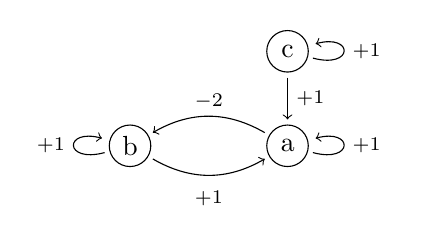
\begin{tikzpicture}[grn]
  \path[use as bounding box] (-1.3,-0.75) rectangle (3.5,1.5);
  \node[inner sep=0] (a) at (2,0) {a};
  \node[inner sep=0] (b) at (0,0) {b};
  \node[inner sep=0] (c) at (2,1.2) {c};
  \path[->]
    (b) edge[bend right] node[elabel, below=-2pt] {$+1$} (a)
    (c) edge node[elabel, right=-2pt] {$+1$} (a)
    (a) edge[bend right] node[elabel, above=-5pt] {$-2$} (b)
    (b) edge[in=-15+180, out=15+180, loop] node[elabel, left=-2pt] {+1} (b)
    (c) edge[in=15, out=-15, loop] node[elabel, right=-2pt] {+1} (c)
    (a) edge[in=15, out=-15, loop] node[elabel, right=-2pt] {+1} (a);
\end{tikzpicture}
}
\caption{\label{fig:BRN-inf1}
  Result of the IG inference performed on the PH of \pref{fig:runningPH-2}.
}
\end{figure}

If we add the action $\PHfrappe{a_2}{b_0}{b_1}$ to the PH of \pref{fig:runningPH-2},
then two unsigned edges towards $b$ are inferred instead of the previous signed edges:
\begin{align*}
  E_+ &= \{\GRNedgef{b}{+}{1}{a}, \GRNedgef{c}{+}{1}{a}, \GRNedgef{a}{+}{1}{a}, \GRNedgef{c}{+}{1}{c}\}\\
  E_- &= \emptyset \qquad\qquad\qquad\qquad
  E_\uns = \{\GRNedgef{a}{\uns}{2}{b}, \GRNedgef{b}{\uns}{1}{b}\}
\end{align*}
This is due to the fact that the actions $\PHfrappe{a_2}{b_1}{b_0}$ and $\PHfrappe{a_2}{b_0}{b_1}$
introduce an oscillation only caused by $a$, which cannot be represented in Thomas modeling.

% vi:spell spelllang=en:
\section{Parametrization inference}\label{sec:infer-K}

\modLP{
Given a PH and an IG (either arbitrary, or inferred following the previous section), this section
addresses the identification of the parametrization for the corresponding Thomas model.}

\modLP{
As described in \pref{ssec:infer-K}, this identification relies on the computation of the focal
processes for each configuration of the parameters.
When there is a unique focal process of a component for a given configuration of its regulators,
the focal process matches with the value of the associated Thomas's parameter.}

\modLP{
However, in the general case, as described in \pref{sec:tr2global} and even when the PH is
well-formed for parameter inference (characterized in the next subsection by \pref{pro:wf-ph-K}),
there may be several focal processes (nondeterministic behavior) or none (cyclic behavior).  Such
a case occurs notably when the PH encodes the union of several Boolean or discrete networks, as
described in \cite{PMR10-TCSB,PCFMR14-chapterLMBS}.}

\modLP{
Hence, we propose in \pref{ssec:admissible-K} the notion of \emph{compatible} parametrization with respect
ot the PH dynamics: a Thomas model is compatible with a PH if its dynamics is included in the PH
dynamics, \ie all the transitions in the Thomas model are possible transitions in the PH.
This relaxed notion of parameterization compatibility allows to enumerate all parametrizations
compatible with a given PH, \ie all Thomas model whose dynamics is included in the PH dynamics.}


\subsection{Parameters inference}\label{ssec:infer-K}

This subsection addresses the inference of independent discrete parameters from a given PH.
The inference is equivalent to the one in \cite{PMR10-TCSB}.
In addition, we characterize the well-formed PH for parameter inference property (\pref{pro:wf-ph-K}),
which implies that %the inferred IG does not contain any unsigned interactions, and thus can be seen as the
%regular IG $(\Gamma, E)$,
%and that 
any process in $\levels{b}{a}$ (resp. $\ulevels{b}{a}$) share the same behavior regarding $a$.

\begin{property}[Well-formed PH for parameter inference]\label{pro:wf-ph-K}
A PH is well-formed for parameter inference if and only if
it is well-formed for BRN identification (\pref{pro:wf-ph}) and
that the associated IG $(\Gamma, E)$ verifies that:
\modLP{
\begin{align}
\begin{split}
\forall b\rightarrow a&\in E, b\neq a,
	\forall \sigma\in L(\PHpredecgene{a}),\\
    \forall (i,j & \in \levels{b}{a} \vee i,j \in \ulevels{b}{a}),
	\forall a_k \in L_a,
	\\
&	\focals(a,\{a_k\},\ctx_a^{\PHpredecgene{a}}(\sigma\{b_i\}))
	=\focals(a,\{a_k\},\ctx_a^{\PHpredecgene{a}}(\sigma\{b_j\}))
\end{split}
\\
\begin{split}
\forall a\in\Gamma, &\forall b\in\PHpredecgene{a},
b\neq a \wedge b\rightarrow a\notin E,\\
	\forall \sigma&\in L(\PHpredecgene{a}), 
    \forall b_i,b_j \in L_b,
	\forall a_k \in L_a,
	\\
&	\focals(a,\{a_k\},\ctx_a^{\PHpredecgene{a}}(\sigma\{b_i\}))
	=\focals(a,\{a_k\},\ctx_a^{\PHpredecgene{a}}(\sigma\{b_j\}))
\end{split}
\end{align}
}
\end{property}

Let $K_{a,\omega}$ be a Thomas's parameter for a given component $a \in \Gamma$ 
with $\omega \subset \GRNreg{a}$ a set of its regulators.
As described in \pref{ssec:thomas}, $K_{a,\omega}$ specifies to which values $a$ eventually evolves
in the configuration matching with $\omega$.

\modLP{The configuration of the PH corresponding to $\omega$ is given as follows.
For each component $b \in \GRNreg{a}$, we define $\sigma^b_{a,\omega}$ (\pref{eq:param_context}) as 
the process of $b$ with the level in 
$\levels{b}{a}$ if $b\in\omega$, or in $\ulevels{b}{a}$ if $b\notin\omega$.
Because of \pref{pro:wf-ph-K}, if several possible levels exist, this process can be chosen
arbitrarily.
If $b$ does not regulate $a$ in the IG, all processes of sort $b$ should have the same action on
$a$, so the process $b_0$ is arbitrarily selected (\pref{eq:param_context_free}).
The configuration $\sigma_{a,\omega}$ corresponding to $\omega$ (\pref{eq:K-ctx})
is then obtained by extending the configuration of the
regulators of $a$ to the (deterministic) cooperative sorts (\pref{def:ctx-sigma} in
\pref{ssec:split-sorts}).
Finally, we denote by $S_a(\sigma)$ (\pref{eq:K-domain}) the set of processes of sort $a$ that are
compatible with a configuration $\sigma$: if $a$ is specified in $\sigma$, then $S_a(\sigma) = \{a_i\}$
where $a_i\in\sigma$; otherwise $S_a(\sigma)$ \modMF{is the set of all processes of sort $a$, that is,} $L_a$.}
\begin{align}
  \label{eq:param_context}
  \forall b\rightarrow a\in E,~
  \sigma_{a,\omega}^b & \DEF \begin{cases}
    \modLP{\min}(\levels{b}{a}) & \text{if $b \in \omega$,}\\
    \modLP{\min}(\ulevels{b}{a}) & \text{if $b \notin \omega$}
  \end{cases}
  \\
  \modLP{
  \forall b\in\PHpredecgene a, b\rightarrow a\notin E,~
  \sigma_{a,\omega}^b} & \modLP{\DEF b_0}
  \label{eq:param_context_free}
  \\
  \sigma_{a,\omega} & \DEF
  \modLP{\ctx_a^{\PHpredecgene{a}}(
  	\state{\sigma^b_{a,\omega} \mid  b\in\PHpredecgene{a}})}
  \label{eq:K-ctx}
  \\
  \modLP{
  \forall a\in\Gamma,~
  S_a(\sigma)} &\modLP{\DEF
	\begin{cases}
	\{a_i\} & \text{if }a_i\in \sigma\\
	L_a & \text{otherwise.}
	\end{cases}}
\label{eq:K-domain}
\end{align}

Therefore, we obtain that
\modLP{$K_{a,\omega} = \focals(a,S_a(\sigma_{a,\omega}),\sigma_{a,\omega})$ if this latter is
a singleton, denoting a deterministic behavior (\pref{pps:param_K})}.

\begin{proposition}[Parameter inference]
\label{pps:param_K}
Let $(\PHs, \PHl, \PHh)$ be a Process Hitting \modLP{with $\PHs=\Gamma\cup\CSorts$} and an
associated IG $\IG = (\Gamma, E)$ well-formed for parameter inference.
For all $a\in\Gamma$, for any $\omega\subseteq \GRNreg{a}$,
if $\focals(a,S_a(\sigma_{a,\omega}),\sigma_{a,\omega})= \{ a_i \}$, then \modLP{$K_{a,\omega} = i$}.
\end{proposition}

\modMF{
\begin{example}
\label{ex:infer-param-runningPH-2}
When applied to the refined PH of \pref{fig:runningPH-2},
and using the IG of \pref{fig:runningBRN}(left)
which is the result of the IG inference on this PH model
(as explained in \pref{ssec:infer-ig-examples}),
\pref{pps:param_K} infers the parametrization of \pref{fig:runningBRN}(right).
The inference of parameters thus finds back all parameters
of the original model when the cooperations are fully defined.
\end{example}
}

\modMF{
\begin{example}
\label{ex:infer-param-runningPH-1}
Regarding the non-refined PH of \pref{fig:runningPH-1},
and using the same IG of \pref{fig:runningBRN}(left),
the parameters of \pref{fig:runningBRN}(right) are inferred,
except the parameters $K_{a,\{b\}}$ and $K_{a,\{c\}}$
for which \pref{pps:param_K} is not conclusive.
The obtained parametrization is therefore partial.
This is due to the lack of precision in the cooperation between $b$ and $c$,
caused by the absence of the cooperative sort.
\end{example}
}

Given the \pref{pps:param_K}, we see that in some cases, the inference of the targeted parameter is impossible.
This can be due to a lack of cooperation between regulators:
when two regulators independently hit a component, their actions can have opposite effects, leading to two possible evolutions.
Such an indeterminism is not possible in Thomas modeling as in a given configuration of regulators,
a component can only have an interval attractor, and can therefore evolve in only one direction.
In order to avoid such inconclusive cases, one has to ensure that no such behavior is allowed by
either removing undesired actions or using cooperative sorts to prevent opposite influences between
concurrent regulators.

\subsection{Admissible parametrizations}\label{ssec:admissible-K}

When building a BRN, one has to find the parametrization that best describes the desired behavior of the studied system.
Complexity is inherent to this process as the number of possible parametrizations for a given IG is exponential w.r.t.~the number of components.
However, the method of parameters inference presented in this section gives some information about necessary parameters given a certain dynamics described by a PH.
This information thus drops the number of possible parametrizations, allowing to find the desired behavior more easily.

We first delimit the validity of a parameter (\pref{pro:K-valid}) in order to ensure that any
transition in the resulting BRN is allowed by the studied PH.
This is verified by the existence of a hit making the concerned component bounce into the direction
of the value of the parameter in the matching context.
Thus, assuming \pref{pro:wf-ph-K} holds, any transition in the inferred BRN corresponds to at least
one transition in the PH, proving the correctness of our inference.
\modMF{%
Any parameter that does not satisfy \pref{pro:K-valid} is therefore excluded from the enumeration.
}%
We remark that all parameters inferred by \pref{pps:param_K} satisfy this property.

\begin{property}[Parameter validity]\label{pro:K-valid}
A parameter $K_{a,\omega}$ is valid w.r.t.~the PH if and only if the following equation is verified:
\begin{align*}
  \forall a_i \in C^a_{a,\omega}, a_i \neq K_{a,\omega} \Longrightarrow
    (& \exists \PHfrappe{c_k}{a_i}{a_j}\in\PHa, c_k \in C^c_{a,\omega} \\
     & \wedge a_i < K_{a,\omega} \Rightarrow j > i \wedge  a_i > K_{a,\omega} \Rightarrow j <i )
\end{align*}
\end{property}

Then, we use some additional biological constraints on Thomas's parameters given in
\cite{BernotSemBRN}, that we sum up in the following three properties:

\begin{property}[Extreme values assumption]
\label{pro:param_enum_extreme}
Let $\IG = (\Gamma, E)$ be an IG. A parametrization $K$ on $\IG$ satisfies the \emph{extreme values assumption} if and only if:
\begin{align*}
  \forall b \in \Gamma, \GRNreg{b} \neq \emptyset \Longrightarrow
    \exists \omega \subset \GRNreg{b}, K_{b,\omega} = 0 \wedge
    \exists \omega' \subset \GRNreg{b}, K_{b,\omega'} = l_b
\end{align*}
\end{property}

\begin{property}[Activity assumption]
\label{pro:param_enum_activity}
Let $\IG = (\Gamma, E)$ be an IG. A parametrization $K$ on $\IG$ satisfies the \emph{activity assumption} if and only if:
\begin{align*}
  \forall b \in \Gamma, \forall a \in \GRNreg{b}, \exists \omega \subset \GRNreg{b}, K_{b,\omega} \neq K_{b,\omega \cup \{ a \}}
\end{align*}
\end{property}

\begin{property}[Monotonicity assumption]
\label{pro:param_enum_monotonicity}
Let $\IG = (\Gamma, E)$ be an IG. A parametrization $K$ on $\IG$ satisfies the \emph{monotonicity assumption} if and only if:
\begin{align*}
  \forall b \in \Gamma,
  \forall A^+ \subset \{ a \in \Gamma \mid \GRNedge{a}{+}{t}{b} \in E_+ \}&,
  \forall A^- \subset \{ a \in \Gamma \mid \GRNedge{a}{-}{t}{b} \in E_- \},\\
  K_{b,\omega \cup A^-} & \leq K_{b,\omega \cup A^+}
\end{align*}
\end{property}

\begin{example}\label{ex:enum-param-runningPH-1}
The parametrization inferred in \pref{ex:infer-param-runningPH-1} was partial
because \modMF{$K_{a,\{b\}}$ and $K_{a,\{c\}}$} could not be inferred.
It is however possible to enumerate all admissible parametrizations
compatible with both the inferred parameters, and the properties of this subsection.
This enumeration gives 9 different parametrizations
which correspond to the 3 possible values
\modMF{%
for both $K_{a,\{b\}}$ and $K_{a,\{c\}}$:
%\[(K_{a,\{b\}}; K_{a,\{c\}}) \in \{ 0, 1, 2 \} \times \{ 0, 1, 2 \}\]
\[K_{a,\{b\}} \in \{ 0, 1, 2 \} \qquad \text{and} \qquad K_{a,\{c\}} \in \{ 0, 1, 2 \}\]
We note that all these solutions satisfy Properties
\ref{pro:K-valid} to \ref{pro:param_enum_monotonicity}.
All the parametrizations obtained from these combinations are thus admissible.
}

Finally, we note that the value \modMF{$1$} belongs to the possible values for both parameters.
Therefore this enumeration allows, from the model in \pref{fig:runningPH-1},
to find the behavior of the model refined with a cooperative sort described in
\pref{fig:runningPH-2}.
\end{example}

\section{Answer Set Programming implementation concepts}\label{sec:impl}

%\newcommand{\atom}{\mathbf}
\newcommand{\atom}[1]{#1}
%\newcommand{\predicate}{\mathbf}
\newcommand{\predicate}[1]{\mathit{#1}}
\newcommand{\la}{\leftarrow}
\newcommand{\var}[1]{#1}
\newcommand{\nota}{\neg}

\newcommand{\paramlabel}{\predicate{param\_label}}
\newcommand{\paramres}{\predicate{param\_resource}}
\newcommand{\component}{\predicate{component}}
\newcommand{\componentlevels}{\predicate{component\_levels}}
\newcommand{\param}{\predicate{param}}
\newcommand{\inferedparam}{\predicate{infered\_param}}
\newcommand{\lessactive}{\predicate{less\_active}}
\newcommand{\paraminf}{\predicate{param\_inf}}



Answer Set Programming (ASP) is a logic programming paradigm \cite{Baral03, Baral10},
which has been chosen to address the enumeration of all admissible parametrizations.
The motivations are following:
\begin{itemize}
  \item ASP efficiently tackles the inherent complexity of the used models, thus enabling us fast execution of the formal tools defined in this paper,
  \item ASP can efficiently enumerate a large set of possible answers,
  \item and it is easy to constrain the answers according to some properties.
\end{itemize}
We now synthesize some key points to better make the reader understand our ASP implementation with the enumeration example.



\subsection{Simple rules and answer sets}\label{sssec:simple_rules}
ASP is based on a set of rules of of the form:
\begin{align*}
  \underbrace{{\ }\atom{H}_{\ }}_{head} \la \underbrace{\atom{A}_1, \atom{A}_2, \dots, \atom{A}_n, \nota \atom{B}_1, \nota \atom{B}_2, \dots, \nota \atom{B}_m}_{body}.
\end{align*}
where the $body$ is a series of atoms ($\atom{A}_i$) and negations of atoms ($\nota \atom{B}_i$).
In the case of \emph{simple rules} (as opposed to the \emph{cardinality rules} of \pref{sssec:cardinality_rules}), the $head$ is also an atom ($\atom{H}$).
Such a rule, whose formal semantics is defined below,
schematically states that if all atoms $\atom{A}_1, \atom{A}_2, \dots, \atom{A}_n$ are true
and all atoms $\atom{B}_1, \atom{B}_2, \dots, \atom{B}_m$ are not true (negation by failure), then $\atom{H}$ has to be true.

An atom is composed of a predicate and a series of arguments (possibly empty).
For example, the following atom:
\begin{align*}
  \predicate{p}(x_1, x_2, \dots, x_r)
\end{align*}
is composed of the predicate $\predicate{p}$ and $r$ arguments: $x_1, x_2, \dots, x_r$.
Each argument is either a \emph{constant}, which is a representation of a piece of data (component name, expression level, …),
or a \emph{variable}, which is in fact a shorthand for any possible constants (variables are detailed below).
In this paper, constants are either numerical or consist of a single lowercase letter (e.g.~$a$, $b$, $c$, $1$, $2$, …)
while variables are always denoted by a single capital letter (e.g.~$\var{A}$, $\var{P}$, $\var{Q}$, …).
We do not use function symbols as arguments in this work.

\begin{example}\label{ex:asp-atom}
Consider a PH model such as depicted in \pref{fig:runningPH-1}:
in order to state the existence of each component, we use a predicate called $\component$ with two arguments:
\begin{align*}
  &\component(x, n).
\end{align*}
where $x$ is the name of the component and $l_x = n$ is its maximum expression level.
\end{example}

An ASP program is a set of rules as described above.
Solving an ASP program means finding an \emph{answer set}, which is a minimal set of atoms that respect all the rules.
In order to formally define this notion of answer set,
let us define a \emph{definite rule} as a rule with no negation of atoms (noted “$\nota$” above),
and a \emph{definite program} as a program containing only definite rules.
Let $S$ be a set of atoms: a definite rule is \emph{satisfied} by $S$ if $\atom{H} \in S$,
or if $\exists i \in \segm{1}{n}, A_i \notin S$.
Given this definition of satisfaction, we define the answer set of a definite program $\Pi$
as the (unique) minimal set $S$ of atoms that satisfies all the rules in $\Pi$.

In order to consider the general case,
for all non-definite program $\Pi$ and set $S$ of atoms, we denote $\Pi^S$ the reduct of $\Pi$ w.r.t.~$S$, defined from $\Pi$ by:
\begin{enumerate}
  \item deleting all the rules that have a negation of atom $\nota \atom{B}_i$ in the body where $\atom{B}_i \in S$, and
  \item removing all negations of atoms in the bodies of the remaining rules.
\end{enumerate}
Then, a set of atoms $S$ is an answer set of a non-definite program $\Pi$ if it is the answer set of $\Pi^S$, which is a definite program.
We note that several answer sets can be solution to the same non-definite program, and in practice a solver can be directed to enumerate them all.

%\begin{example}
%  As an example not related to the current work, consider the following ASP program:
%  \begin{align*}
%    a &\la \nota b.\\
%    b &\la \nota a.
%  \end{align*}
%  This program has the two following answer sets: $\{a\}$ and $\{b\}$.
%\end{example}



Note that it is possible to define a simple rule with no $body$ part.
Such a rule is called a \emph{fact}, and its $head$ atom consequently has to belong to all answer sets.
For instance, the information describing the studied model (the original PH model and the inferred IG and parameters) are expressed in ASP using facts.

\begin{example}\label{ex:asp-component}
In order to define the 3 components of \pref{fig:runningPH-1}, we use the following program:
\begin{align*}
  &\component(a, 2). \\
  &\component(b, 1). \\
  &\component(c, 1).
\end{align*}
This program contains only facts using the predicate $\component$ defined in \pref{ex:asp-atom},
and $a$, $b$, $c$, $1$ and $2$ are constants.
\end{example}



\subsection{Variables}
To describe the sets of all expression levels of each component (\ie the set $\segm{0}{l_a}$ for each $a \in \Gamma$),
one can use atoms of the form $\componentlevels(a, k)$ to state that $k \in \segm{0}{l_a}$.
Variables here come in handy to enumerate each possible constant $k$ for each component $a$:
before solving, any rule containing variables is \emph{grounded}, that is, replaced by an equivalent set of rules with constants only.
%during the solving, any rule containing variables is duplicated in order to replace each variable by all the possible constants it could represent.
The following rule, for example, contains three variables ($\var{A}$, $\var{K}$ and $\var{M}$) and enumerates the set of possible expression levels of each component in the system:
\begin{align*}
  \componentlevels(A, K) \la \component(\var{A}, \var{M}), 0 \leq K \leq M.
\end{align*}
where the notation “$\leq$” stands for a shortcut in ASP which has the same meaning as the mathematical operator.

\begin{example}
Regarding \pref{fig:runningPH-1}, the previous rule together with the facts of \pref{ex:asp-component}
will give the following answer set:
\begin{align*}
  &\{&&\component(a, 2),
  &&\component(b, 1), \\
  &&&\component(c, 1),
  &&\componentlevels(a, 0), \\
  &&&\componentlevels(a, 1),
  &&\componentlevels(a, 2), \\
  &&&\componentlevels(b, 0),
  &&\componentlevels(b, 1), \\
  &&&\componentlevels(c, 0),
  &&\componentlevels(c, 1). &\}
\end{align*}
\end{example}



\subsection{Cardinality rules}
\label{sssec:cardinality_rules}
As an extension of simple rules, \emph{cardinality rules} turn out to be convenient to enumerate a set of answer sets.
The head of a cardinality rule specifies a set of atoms $H$ and two integers $min$ and $max$, and is denoted:
\begin{align*}
  min\ \{\ H\ \}\ max \la \atom{A}_1, \atom{A}_2, \dots, \atom{A}_n, \nota \atom{B}_1, \nota \atom{B}_2, \dots, \nota \atom{B}_m.
\end{align*}
Given such a rule, as many answer sets as possible are created, so that each answer set $S$ verifies:
\begin{align*}
  min \leq |S \cap H| \leq max
\end{align*}
and every atom $\atom{H}_i \in S \cap H$ respects the simple rule:
\begin{align*}
  \atom{H}_i \la \atom{A}_1, \atom{A}_2, \dots, \atom{A}_n, \nota \atom{B}_1, \nota \atom{B}_2, \dots, \nota \atom{B}_m.
\end{align*}
In other words, all answer sets contain a subset of $H$ whose cardinality goes from $min$ to $max$,
and for which the condition in the body of the cardinality rule is met.
The set of atoms $H = \{ \atom{H}_1, \atom{H}_2, \dots, \atom{H}_p \}$ is often defined as: $H = \{ \atom{P} \mid \atom{Q} \}$,
which is a shorthand for “the set of atoms of the form $\atom{P}$ for which $\atom{Q}$ is true”.

Cardinality rules turn out to be convenient to enumerate all possible parametrizations by creating multiple answer sets.
For functional purposes, a unique label is assigned to every possible set of resources of a given component.
Thus, we denote $\omega_p$ the set of resources of a given component $a$ labeled by $p$,
and naturally, $K_{a,\omega_p}$ is the related parameter.
%and in the following we note $K_{a,\omega_p}$ the parameter of component $a$ whose set of resources $\omega$ is assigned to the label $p$.
We note that labeling the sets of resources of a component is obviously equivalent to labeling its parameters.
Then, suppose that:
\begin{itemize}
  \item $\paramlabel(a, p)$ states that $p$ is a valid label for a set of resources of component $a$ (and therefore $K_{a,\omega_p}$ is a valid parameter);
  \item $\param(a, p, i)$ states that: $K_{a, \omega_p} = i$;
  \item $\inferedparam(a, p)$ states that the parameter inference of $K_{a, \omega_p}$ was conclusive (\pref{pps:param_K}).
\end{itemize}
It is thereby possible to enumerate the possible values of all parameters for which \pref{pps:param_K} was not conclusive, with the following cardinality rule:
\begin{align*}
  & 1\ \{\ \param(\var{A}, \var{P}, \var{I}) \mid \componentlevels(\var{A}, \var{I})\ \}\ \modMF{1}\ \la \\
  & \qquad\qquad\qquad \paramlabel(\var{A}, \var{P}), \nota \inferedparam(\var{A}, \var{P}).
\end{align*}
Indeed, this rule applies to any possible parameter $\var{P}$ of any component $\var{A}$ ($\paramlabel$) whose value is still unknown ($\nota \inferedparam$),
and states that any expression level $\var{I}$ of this component ($\componentlevels$)
is a candidate value for the parameter ($\param$).
\modMF{
Furthermore, both the lower and upper bounds are $1$,
which forces each enumerated parameter to have exactly one value.
}
%but no upper bound is specified ($\infty$) for the size of each parameter
%(which is in fact already bounded by the number of possible expression levels of the related component).
%each parameter contains at least $1$ value, as stated by the lower bound, and has no upper bound ($\infty$) but the number of expression levels of its component.
In other worlds, this cardinality rule creates as many answer sets as there are \emph{candidate} parametrizations
so that if $K_{a, \omega_p}$ could not be inferred by \pref{pps:param_K}, then
\modMF{
$K_{a, \omega_p} \in \segm{0}{l_a}$
}
(thus completely disregarding the notion of admissible parametrizations given in \pref{ssec:admissible-K}).



\begin{example}\label{ex:cardinality}
\modMF{%
In the scope of \pref{ex:infer-param-runningPH-1},
$K_{a,\{b\}}$ and $K_{a,\{c\}}$
could not be inferred by \pref{pps:param_K}.
The previous cardinality rule allows to produce 9 parametrizations,
in which these three parameters can take all possible values:
%(as, in this case, the assumptions of \pref{ssec:admissible-K} bring no new constraint):
\begin{align*}
  (K_{a,\{b\}}; K_{a,\{c\}}; K_{b,\emptyset}) \in
    \{ 0, 1, 2 \} \times \{ 0, 1, 2 \}
\end{align*}
and all the other parameters keep their inferred values.
%These parametrizations take the form of sets of $\param$ atoms.
% Note that $\{ 0, 2 \}$ belongs to the set of candidate parametrizations
% as no rule specifying that a parameter has to be an interval has been defined yet.
}%
\end{example}



\subsection{Constraints}\label{sssec:constraints}
Finally, a \emph{constraint} is a rule with no $head$ part:
\begin{align*}
  \la \atom{A}_1, \atom{A}_2, \dots, \atom{A}_n, \nota \atom{B}_1, \nota \atom{B}_2, \dots, \nota \atom{B}_m.
\end{align*}
A constraint is satisfied only if its $body$ is not satisfied,
which thus allows to invalidate answer sets containing some unwanted combinations of atoms.
In the scope of parameters enumeration, for example, constraints are especially useful
to filter out parametrizations that do not respect the assumptions of \pref{ssec:admissible-K}.
Indeed, suppose that:
\begin{itemize}
  \item $\lessactive(a, p, q)$ states that $\omega_p$ is a set of resources of $a$ with (loosely) less activators and more inhibitors than $\omega_q$;
  \item $\paraminf(a, p, q)$ states that: $K_{a,\omega_p} \leq K_{a,\omega_q}$.
\end{itemize}
Then, the monotonicity assumption (\pref{pro:param_enum_monotonicity}) is formulated as the following constraint:
\begin{align*}
  \la \lessactive(\var{A}, \var{P}, \var{Q}), \nota \paraminf(\var{A}, \var{P}, \var{Q}).
\end{align*}
Indeed, this constraint removes all parametrization results where parameters $K_{\var{A},\omega_\var{P}}$ and $K_{\var{A},\omega_\var{Q}}$ exist
such that $\var{A}$ is less activated by the set of resources $\omega_\var{P}$ than it is by $\omega_\var{Q}$,
but $K_{\var{A},\omega_\var{Q}} < K_{\var{A},\omega_\var{P}}$,
thus violating the monotonicity assumption.
Of course, other assumptions can be formulated in the same way.

% \begin{example}
% \modMF{%
% The set of candidate values given in \pref{ex:cardinality} can be filtered using constraints.
% % For example, a constraint was written in order to obtain only interval parameters
% % (thus avoiding parameters with “gaps” such as $\{ 0, 2 \}$).
% % Applying such a constraint would reduce the set of possible values for the parameters $K_{a,\{a,b\}}$ and $K_{a,\{a,c\}}$ to:
% % \begin{align*}
% %   (K_{a,\{a,b\}} ; K_{a,\{a,c\}}) \in \{ \segm{0}{0} , \segm{1}{1} , \segm{2}{2} , \segm{0}{1} , \segm{1}{2} , \segm{0}{2} \}^2
% % \end{align*}
% % }%
% % 
% % \modMF{%
% }%
% \todo{Find an example to apply the monotonicity assumption?}
% \end{example}
\todo{Find an example to apply the filtering?}



\medskip

This subsection succinctly described how ASP programs come in handy to represent a model and solve complex problems on it.
%all steps of Thomas' modeling inference.
It finds a particularly interesting application in the enumeration of parameters:
all possible parametrizations are generated in separate answer sets,
and integrity constraints are formulated to remove those that do not fit the assumptions of admissible parametrizations,
thus reducing the number of candidate parametrizations to be considered in the end.
However, all steps of the inference presented in this paper (\pref{sec:infer-IG} \& \ref{sec:infer-K})
were implemented in and benefited from this programming paradigm.
%, although in significantly different ways.

\input{parts-example}
\section{Conclusion and Discussion}

This work establishes the abstraction relationship between PH and Thomas's approaches for
qualitative BRN modeling.
The PH allows an abstract representation of BRNs dynamics (allowing incomplete knowledge on the
cooperation between components) that cannot be exactly represented in Ren\'e Thomas's formalism by a
single instance of BRN parametrization.
This motivates the concretization of PH models into a set of compatible Thomas models in order to benefit
of the complementary advantages of these two formal frameworks.

We first propose an original inference of the Interaction Graph (IG) from a BRN
having its dynamics specified in the PH framework.
An IG gives a compact abstract representation of the influence of the components between each
others.
Then, based on a prior inference of Ren\'e Thomas's parametrization for BRNs from a PH model, we
delimit the set of admissible Thomas's parametrizations that are compatible with the PH dynamics,
and give arguments for their correctness.
A parametrization is compatible with the PH if its dynamics (in terms of possible transitions) is included in the PH dynamics.
The enumeration of such parametrizations is efficiently tackled using Answer Set Programming.
We illustrate the overall method with several results
on \modMF{both small and} large biological models.

Several extensions of the presented work are now to be considered.
First, the link between successively refined models of a system could be formally studied.
Indeed, it is convenient to refine a PH model by removing actions or adding cooperations;
the study and formalization of such process would allow to predict behavioral changes and lead to more accurate models.
Second, the inference of BRN multiplexes \cite{BernotMultiplexes} may be of practical interest 
as they allow to implicitly reduce the possible parametrizations by making cooperations appear
in the IG.
Because of its atomicity, the PH allows to specify a range of cooperations that cannot be
completely captured by a single instance of BRN multiplexes, then encouraging the inference of a set
of compatible ones.
Finally, in order to improve the performances in the IG inference, we will consider projection operations on
the PH structure to undo cooperations between components and reduce the cardinality of
configurations to explore by making the interactions independent.

\paragraph{Acknowledgement}
This work was partially supported by the Fondation Centrale Initiatives and
the French National Agency for Research (ANR-10-BLANC-0218 BioTempo project).



\bibliographystyle{elsarticle-num}
\bibliography{biblio}

\appendix

\section*{Appendix.
  List of actions of the phage lambda immunity control model used in \pref{ssec:phage-lambda}}


\begin{align*}
\PHh = \{ \qquad
  \PHfrappe{\cI_0}{\cIcro_0}{\cIcro_2} &&
  \PHfrappe{\cI_0}{\cIcro_1}{\cIcro_3} \\
  \PHfrappe{\cI_0}{\cro_0}{\cro_1} &&
  \PHfrappe{\cI_0}{\cro_1}{\cro_2} \\
  \PHfrappe{\cI_0}{\cro_2}{\cro_3} &&
  \PHfrappe{\cI_1}{\cIcro_0}{\cIcro_2} \\
  \PHfrappe{\cI_1}{\cIcro_1}{\cIcro_3} &&
  \PHfrappe{\cI_1}{\cIcro_2}{\cIcro_0} \\
  \PHfrappe{\cI_1}{\cIcro_3}{\cIcro_1} &&
  \PHfrappe{\cI_1}{\cro_0}{\cro_1} \\
  \PHfrappe{\cI_1}{\cro_1}{\cro_2} &&
  \PHfrappe{\cI_1}{\cro_2}{\cro_3} \\
  \PHfrappe{\cI_2}{\cIcro_2}{\cIcro_0} &&
  \PHfrappe{\cI_2}{\cIcro_3}{\cIcro_1} \\
  \PHfrappe{\cI_2}{\cro_1}{\cro_0} &&
  \PHfrappe{\cI_2}{\cro_2}{\cro_1} \\
  \PHfrappe{\cI_2}{\cro_3}{\cro_2} &&
  \PHfrappe{\cIcro_0}{\cIcroN_2}{\cIcroN_0} \\
  \PHfrappe{\cIcro_0}{\cIcroN_3}{\cIcroN_1} &&
  \PHfrappe{\cIcro_0}{\N_1}{\N_0} \\
  \PHfrappe{\cIcro_1}{\cIcroN_2}{\cIcroN_0} &&
  \PHfrappe{\cIcro_1}{\cIcroN_3}{\cIcroN_1} \\
  \PHfrappe{\cIcro_1}{\N_1}{\N_0} &&
  \PHfrappe{\cIcro_2}{\cIcroN_2}{\cIcroN_0} \\
  \PHfrappe{\cIcro_2}{\cIcroN_3}{\cIcroN_1} &&
  \PHfrappe{\cIcro_2}{\N_1}{\N_0} \\
  \PHfrappe{\cIcro_3}{\cIcroN_0}{\cIcroN_2} &&
  \PHfrappe{\cIcro_3}{\cIcroN_1}{\cIcroN_3} \\
  \PHfrappe{\cIcro_3}{\N_0}{\N_1} &&
  \PHfrappe{\cIcroN_0}{\cII_1}{\cII_0} \\
  \PHfrappe{\cIcroN_1}{\cII_1}{\cII_0} &&
  \PHfrappe{\cIcroN_2}{\cII_1}{\cII_0} \\
  \PHfrappe{\cIcroN_3}{\cII_0}{\cII_1} &&
  \PHfrappe{\cII_0}{\crocII_0}{\crocII_1} \\
  \PHfrappe{\cII_0}{\crocII_2}{\crocII_3} &&
  \PHfrappe{\cII_1}{\crocII_1}{\crocII_0} \\
  \PHfrappe{\cII_1}{\crocII_3}{\crocII_2} &&
  \PHfrappe{\cro_0}{\cIcro_0}{\cIcro_1} \\
  \PHfrappe{\cro_0}{\cIcro_2}{\cIcro_3} &&
  \PHfrappe{\cro_0}{\crocII_2}{\crocII_0} \\
  \PHfrappe{\cro_0}{\crocII_3}{\crocII_1} &&
  \PHfrappe{\cro_1}{\cIcro_0}{\cIcro_1} \\
  \PHfrappe{\cro_1}{\cIcro_2}{\cIcro_3} &&
  \PHfrappe{\cro_1}{\crocII_0}{\crocII_2} \\
  \PHfrappe{\cro_1}{\crocII_1}{\crocII_3} &&
  \PHfrappe{\cro_2}{\cIcro_0}{\cIcro_1} \\
  \PHfrappe{\cro_2}{\cIcro_1}{\cIcro_0} &&
  \PHfrappe{\cro_2}{\cIcro_2}{\cIcro_3} \\
  \PHfrappe{\cro_2}{\cIcro_3}{\cIcro_2} &&
  \PHfrappe{\cro_2}{\crocII_0}{\crocII_2} \\
  \PHfrappe{\cro_2}{\crocII_1}{\crocII_3} &&
  \PHfrappe{\cro_3}{\cIcro_1}{\cIcro_0} \\
  \PHfrappe{\cro_3}{\cIcro_3}{\cIcro_2} &&
  \PHfrappe{\cro_3}{\cro_3}{\cro_2} \\
  \PHfrappe{\cro_3}{\crocII_0}{\crocII_2} &&
  \PHfrappe{\cro_3}{\crocII_1}{\crocII_3} \\
  \PHfrappe{\crocII_0}{\cI_0}{\cI_1} &&
  \PHfrappe{\crocII_0}{\cI_1}{\cI_2} \\
  \PHfrappe{\crocII_1}{\cI_0}{\cI_1} &&
  \PHfrappe{\crocII_1}{\cI_1}{\cI_2} \\
  \PHfrappe{\crocII_2}{\cI_0}{\cI_1} &&
  \PHfrappe{\crocII_2}{\cI_1}{\cI_2} \\
  \PHfrappe{\crocII_3}{\cI_1}{\cI_0} &&
  \PHfrappe{\crocII_3}{\cI_2}{\cI_1} \\
  \PHfrappe{\N_0}{\cIcroN_1}{\cIcroN_0} &&
  \PHfrappe{\N_0}{\cIcroN_3}{\cIcroN_2} \\
  \PHfrappe{\N_1}{\cIcroN_0}{\cIcroN_1} &&
  \PHfrappe{\N_1}{\cIcroN_2}{\cIcroN_3} && \}
\end{align*}


\end{document}
